\documentclass[12pt,a4paper,oneside]{article}

% ===================== NGÔN NGỮ VÀ PHÔNG CHỮ =====================
\usepackage{fontspec}
\setmainfont{Times New Roman}
\setsansfont{Arial}
\setmonofont{Consolas}[Scale=0.88]
\usepackage[vietnamese]{babel}

% ===================== BỐ CỤC =====================
\usepackage{geometry}
\geometry{top=2.5cm,bottom=2.5cm,left=3.0cm,right=2.0cm}
\usepackage{setspace}
\setstretch{1.28}
\usepackage{indentfirst}
\setlength{\parindent}{1.0cm}
\setlength{\emergencystretch}{2.5em}

% ===================== TOÁN VÀ ĐỒ HỌA =====================
\usepackage{amsmath,amssymb}
\usepackage{graphicx}
\usepackage{float}
\usepackage{xcolor}
\usepackage{tikz}

% ===================== BẢNG =====================
\usepackage{booktabs}
\usepackage{longtable}
\usepackage{tabularx}
\usepackage{array}
\usepackage{multirow}
\renewcommand{\arraystretch}{1.15}

% ===================== TIÊU ĐỀ, MỤC LỤC =====================
\usepackage{titlesec}
\usepackage{tocloft}
\usepackage{fancyhdr}
\usepackage[font=small,labelfont=bf,justification=justified,singlelinecheck=false,skip=6pt]{caption}

\titleformat{\section}[block]{\centering\bfseries\large}{PHẦN \thesection.}{0.6em}{}
\titlespacing*{\section}{0pt}{0pt}{16pt}
\titleformat{\subsection}[hang]{\bfseries\normalsize}{\thesubsection}{0.6em}{}
\titlespacing*{\subsection}{0pt}{14pt}{6pt}
\titleformat{\subsubsection}[hang]{\itshape\normalsize}{\thesubsubsection}{0.6em}{}
\titlespacing*{\subsubsection}{0pt}{10pt}{4pt}

\renewcommand{\cfttoctitlefont}{\hfill\bfseries\large}
\renewcommand{\cftaftertoctitle}{\hfill}
\renewcommand{\cftloftitlefont}{\hfill\bfseries\large}
\renewcommand{\cftafterloftitle}{\hfill}
\renewcommand{\cftlottitlefont}{\hfill\bfseries\large}
\renewcommand{\cftafterlottitle}{\hfill}
\setlength{\cftsecnumwidth}{2.4em}
\setlength{\cftsubsecnumwidth}{3.0em}
\renewcommand{\cftsecfont}{\bfseries}

\pagestyle{fancy}
\fancyhf{}
\setlength{\headheight}{14pt}
\fancyhead[L]{\small\itshape Đánh giá mã C++ song song do LLM sinh}
\fancyfoot[C]{\small\thepage}
\renewcommand{\headrulewidth}{0.4pt}

% ===================== MÃ NGUỒN =====================
\usepackage{listings}
\lstset{
  language=C++,
  basicstyle=\ttfamily\footnotesize,
  keywordstyle=\color{blue!65!black}\bfseries,
  commentstyle=\color{green!40!black}\itshape,
  stringstyle=\color{red!60!black},
  numbers=left,
  numberstyle=\tiny\color{gray},
  numbersep=8pt,
  frame=single,
  rulecolor=\color{gray!55},
  breaklines=true,
  columns=fullflexible,
  keepspaces=true,
  showstringspaces=false,
  tabsize=2,
  captionpos=b,
  xleftmargin=1.6em,
  framexleftmargin=1.2em,
  aboveskip=8pt,
  belowskip=8pt
}

% ===================== LIÊN KẾT =====================
\usepackage{hyperref}
\hypersetup{
  colorlinks=true,
  linkcolor=black,
  citecolor=black,
  urlcolor=blue!60!black,
  pdftitle={Danh gia ma C++ hien dai va MPI+OpenMP do LLM sinh cho bai toan Mandelbrot},
  pdfauthor={Bao cao Bo mon Tinh toan song song}
}
\usepackage{enumitem}
\setlist[itemize]{topsep=4pt,itemsep=2pt,parsep=0pt}
\setlist[enumerate]{topsep=4pt,itemsep=2pt,parsep=0pt}

% ===================== LỆNH DÙNG NHIỀU =====================
\newcommand{\code}[1]{\texttt{#1}}
\newcommand{\term}[1]{\textit{#1}}
\newcommand{\phant}[1]{\clearpage\section{#1}}

\begin{document}

% ===================== TRANG BÌA =====================
\begin{titlepage}
\thispagestyle{empty}
\begin{tikzpicture}[remember picture,overlay]
  \draw[line width=2.2pt]
    ([xshift=1.25cm,yshift=-1.25cm]current page.north west)
    rectangle
    ([xshift=-1.25cm,yshift=1.25cm]current page.south east);
  \draw[line width=0.6pt]
    ([xshift=1.45cm,yshift=-1.45cm]current page.north west)
    rectangle
    ([xshift=-1.45cm,yshift=1.45cm]current page.south east);
\end{tikzpicture}
\begin{center}
  {\large TRƯỜNG ĐẠI HỌC KHOA HỌC TỰ NHIÊN\par}
  \vspace{2pt}
  {\large\bfseries KHOA TOÁN -- CƠ -- TIN HỌC\par}

  \vspace{0.75cm}
  
\includegraphics[width=2.5cm]{figures/logo.png}\par

  \vspace{1.05cm}
  {\Large BÁO CÁO\par}
  \vspace{4pt}
  {\Large\bfseries BỘ MÔN TÍNH TOÁN SONG SONG\par}

  \vspace{1.1cm}
  {\large Đề tài:\par}
  \vspace{0.45cm}
  {\bfseries\Large ĐÁNH GIÁ MÃ C++ HIỆN ĐẠI VÀ MPI+OPENMP\\
   DO LLM SINH CHO BÀI TOÁN TẬP MANDELBROT\\
   CÓ KHẢ NĂNG MỞ RỘNG\par}
  \vspace{0.4cm}
  {\itshape\small Evaluating LLM-Generated Modern C++ and MPI+OpenMP\\
   Codes for Scalable Mandelbrot Set Computation\par}

  \vspace{1.2cm}
  \begin{tabular}{@{}l@{\hspace{0.5cm}}l@{}}
    Sinh viên thực hiện: & [Họ và tên sinh viên 1] \\[2pt]
                        & [Họ và tên sinh viên 2] \\[0.3cm]
    Giảng viên hướng dẫn: & TS. Nguyễn Hải Vinh \\[2pt]
                          & TS. Mạc Đăng Trường \\
  \end{tabular}

  \vfill
  {\large Hà Nội, 11 -- 2026\par}
  \vspace{0.4cm}
\end{center}
\end{titlepage}

% ===================== PHẦN ĐẦU =====================
\pagenumbering{roman}
\pagestyle{plain}

\tableofcontents
\clearpage

\listoffigures
\clearpage

\listoftables
\clearpage

\section*{DANH MỤC TỪ VIẾT TẮT}
\addcontentsline{toc}{section}{DANH MỤC TỪ VIẾT TẮT}

\begin{center}
\small
\begin{tabularx}{0.92\textwidth}{@{}l X@{}}
\toprule
\textbf{Từ viết tắt} & \textbf{Diễn giải} \\
\midrule
API   & Application Programming Interface -- giao diện lập trình ứng dụng \\
CLI   & Command Line Interface -- giao diện dòng lệnh \\
COCOMO & Constructive Cost Model -- mô hình ước lượng chi phí phần mềm \\
CPU   & Central Processing Unit -- đơn vị xử lý trung tâm \\
HPC   & High-Performance Computing -- tính toán hiệu năng cao \\
I/O   & Input/Output -- vào/ra dữ liệu \\
LLM   & Large Language Model -- mô hình ngôn ngữ lớn \\
LOC   & Lines of Code -- số dòng mã nguồn \\
MPI   & Message Passing Interface -- giao diện truyền thông điệp \\
OpenMP & Open Multi-Processing -- chuẩn lập trình song song bộ nhớ chia sẻ \\
PBM   & Portable Bitmap -- định dạng ảnh bitmap đơn sắc của họ Netpbm \\
PGM   & Portable Graymap -- định dạng ảnh xám của họ Netpbm \\
RQ    & Research Question -- câu hỏi nghiên cứu \\
SPMD  & Single Program, Multiple Data -- một chương trình, nhiều dữ liệu \\
TBB   & Threading Building Blocks -- thư viện song song của Intel \\
\bottomrule
\end{tabularx}
\end{center}

\vspace{0.5cm}
\noindent\textit{Ghi chú:} Báo cáo giữ nguyên tên riêng của các mô hình
(ChatGPT-4, ChatGPT-5, Claude, LLaMA) và tên định danh kỹ thuật
(\code{std::async}, \code{MPI\_Gather}, \code{final\_suspend}, \ldots)
như trong bài báo gốc để bảo đảm khả năng đối chiếu.


% ===================== THÂN BÀI =====================
\clearpage
\pagenumbering{arabic}
\pagestyle{fancy}

\phant{GIỚI THIỆU}\label{sec:gioithieu}

\subsection{Bối cảnh}

Tính toán hiệu năng cao (HPC) được xây dựng trên hai trụ cột lập trình song song:
bộ nhớ chia sẻ (shared memory) và bộ nhớ phân tán (distributed memory). Trong mô
hình thứ nhất, nhiều luồng (thread) cùng truy cập một không gian địa chỉ, phối
hợp với nhau qua biến dùng chung, rào chắn và cơ chế đồng bộ. Trong mô hình thứ
hai, nhiều tiến trình (process) chạy trên các nút khác nhau, trao đổi dữ liệu
bằng thông điệp. Mỗi mô hình có chi phí riêng: đồng bộ và tranh chấp bộ nhớ ở
mô hình chia sẻ; độ trễ và băng thông truyền thông ở mô hình phân tán. Việc viết
mã song song đúng, nhanh và mở rộng được đòi hỏi hiểu biết đồng thời về thuật
toán, kiến trúc máy tính, mô hình bộ nhớ và công cụ biên dịch.

Trong hơn một thập kỷ, chuẩn C++ đã bổ sung dần các cơ chế song song ngay trong
ngôn ngữ: \code{std::thread} và \code{std::async} (C++11), thuật toán song song
với execution policy (C++17), coroutine cùng ranges, semaphore, latch, barrier
(C++20) \cite{diehl2023shared,diehl2024book}. Song song với đó, OpenMP và MPI vẫn
là hai chuẩn thực tế được dùng rộng rãi nhất trong các ứng dụng khoa học. Sự
phong phú này tạo ra nhiều cách diễn đạt cùng một phép song song, nhưng cũng làm
tăng không gian lỗi: một chương trình có thể biên dịch thành công, chạy không
báo lỗi, mà vẫn cho kết quả sai hoặc không hề tận dụng số lõi được yêu cầu.

Cùng lúc đó, các mô hình ngôn ngữ lớn (LLM) đã trở thành công cụ hỗ trợ sinh mã
phổ biến. Từ một mô tả bằng ngôn ngữ tự nhiên, mô hình có thể tạo ra hàm, lớp,
thậm chí cả chương trình hoàn chỉnh. Các đánh giá ban đầu tập trung vào bài toán
lập trình thuật toán hoặc mã tuần tự, nơi tiêu chí đúng/sai tương đối rõ ràng.
Với mã HPC, tiêu chí phức tạp hơn nhiều: ngoài tính đúng, còn có khả năng biên
dịch trên toolchain thực tế, khả năng kiểm soát tài nguyên, tính ổn định khi
tăng số lõi và hiệu năng so với mã do con người viết.

\subsection{Vấn đề nghiên cứu}

Khoảng trống mà bài báo gốc \cite{diehl2026} hướng tới nằm ở giao điểm của ba yếu
tố. Thứ nhất, phần lớn nghiên cứu về LLM sinh mã chỉ đánh giá một mô hình lập
trình đơn lẻ, chẳng hạn OpenMP, OpenACC hoặc MPI, nên thiếu so sánh ngang hàng
giữa các mức trừu tượng. Thứ hai, các nghiên cứu thường dừng ở tỉ lệ biên dịch
hoặc tỉ lệ vượt qua bộ kiểm thử, mà không đo khả năng mở rộng trên phần cứng
song song thật. Thứ ba, kiến thức của LLM về hệ sinh thái công cụ — trình biên
dịch nào, thư viện nền nào, phiên bản chuẩn nào — hầu như chưa được kiểm chứng,
dù đây chính là nguồn lỗi phổ biến trong thực tế.

Bài toán Mandelbrot được chọn làm phép thử có kiểm soát. Đây là bài toán song
song hiển nhiên (\term{embarrassingly parallel}): mỗi điểm ảnh được tính độc lập,
không cần bộ giải, không có trao đổi dữ liệu giữa các đơn vị tính toán. Nhờ vậy,
sai sót quan sát được chủ yếu đến từ cách biểu diễn song song, cách quản lý luồng
và cách xuất kết quả, chứ không bị nhiễu bởi thuật toán số phức tạp. Nói cách
khác, bài toán đóng vai trò một \term{benchmark tối thiểu} để cô lập năng lực sinh
mã song song của LLM.

\subsection{Mục tiêu và câu hỏi nghiên cứu}

Mục tiêu của bài báo là đánh giá một cách có hệ thống bốn LLM hàng đầu
(ChatGPT-4, ChatGPT-5, Claude và LLaMA \cite{achiam2023gpt4,touvron2023llama}) trên năm biến thể lập trình song song:
C++11 bất đồng bộ, C++17 thuật toán song song, C++20 coroutine, OpenMP và
MPI+OpenMP. Ba câu hỏi nghiên cứu được đặt ra:

\begin{enumerate}[label=\textbf{RQ\arabic*.},leftmargin=2.2cm]
  \item LLM sinh mã C++ song song đúng cú pháp và biên dịch được ở mức nào?
  \item Những lỗi thực thi và ngữ nghĩa nào xuất hiện, chúng khó sửa đến đâu, và
        nguyên nhân gốc là gì?
  \item Sau khi sửa, mã sinh ra có mở rộng theo số lõi và số nút không, và có
        cạnh tranh được với mã do con người viết không?
\end{enumerate}

\subsection{Đóng góp}

Bài báo gốc nêu bốn đóng góp: (i) thiết kế prompt có cấu trúc cho C++11/17/20,
OpenMP và MPI+OpenMP, dùng nhất quán cho mọi mô hình; (ii) phân tích chi tiết kết
quả biên dịch, lỗi thực thi và tính đúng chức năng; (iii) đánh giá coroutine
C++20 — cơ chế song song mới nhất, đang được tích hợp vào Kokkos và HPX; (iv)
phân loại lỗi và cách khắc phục, qua đó chỉ ra giới hạn của LLM trong tổng hợp và
gỡ lỗi mã HPC.

Báo cáo này bổ sung thêm ba đóng góp trình bày:

\begin{itemize}
  \item Hệ thống hóa cơ sở lý thuyết của từng mô hình lập trình, giải thích vì sao
        các lỗi quan sát được lại xảy ra ở đúng điểm đó, thay vì chỉ liệt kê triệu
        chứng.
  \item Xây dựng một phân loại lỗi theo tầng (cú pháp, API, ngữ nghĩa, đồng bộ,
        định dạng, đo đạc) kèm mức độ khó sửa và kiến thức cần có.
  \item Chuyển kết quả nghiên cứu thành quy trình kiểm duyệt và danh mục kiểm tra
        thực dụng cho nhóm phát triển HPC có sử dụng LLM hỗ trợ.
\end{itemize}

\subsection{Phạm vi và cách tiếp cận}

Phạm vi thực nghiệm giới hạn ở bốn mô hình ngôn ngữ, năm biến thể lập trình, một
bài toán, một trình biên dịch (GCC 11.5.0), một backend song song (Intel TBB
2022.2) và một cụm CPU. Mỗi biến thể được sinh một lần từ một prompt cố định,
sau đó con người sửa lỗi biên dịch và lỗi thực thi theo cách tối thiểu, ghi nhận
lại từng thay đổi. Kết quả hiệu năng vì thế phản ánh mã \emph{sau khi sửa}, không
phải chất lượng nguyên bản của lần sinh đầu tiên. Cách tiếp cận này phù hợp với
câu hỏi thực tiễn: điều người dùng quan tâm là LLM tạo ra bao nhiêu việc phải sửa
và sau khi sửa thì mã có dùng được không.

\subsection{Bố cục báo cáo}

Phần~\ref{sec:coso} trình bày cơ sở lý thuyết: bài toán Mandelbrot, bốn cơ chế
song song của C++, OpenMP, MPI và mô hình lai, cùng nền tảng về LLM sinh mã.
Phần~\ref{sec:phuongphap} mô tả thiết kế thực nghiệm, prompt, quy trình kiểm định,
độ đo và môi trường đo. Phần~\ref{sec:ketqua} trình bày kết quả theo từng mô hình
và từng biến thể, kèm phân tích lỗi, chất lượng mã và khả năng mở rộng.
Phần~\ref{sec:thaoluan} thảo luận nguyên nhân, hàm ý thực tiễn và hạn chế.
Phần~\ref{sec:ketluan} kết luận và nêu hướng phát triển. Phụ lục cung cấp bảng
tổng hợp lỗi, trích mã tiêu biểu và danh mục kiểm tra.

\phant{CƠ SỞ LÝ THUYẾT}\label{sec:coso}

\subsection{Tập Mandelbrot}

\subsubsection{Định nghĩa và thuật toán thoát}

Tập Mandelbrot được định nghĩa từ phép lặp trên mặt phẳng phức. Với mỗi số phức
$c\in\mathbb{C}$, xét dãy
\begin{equation}
  z_0 = 0, \qquad z_{n+1} = z_n^2 + c, \quad n=0,1,2,\ldots
  \label{eq:mandel}
\end{equation}
Điểm $c$ thuộc tập Mandelbrot nếu dãy $(z_n)$ bị chặn. Người ta chứng minh được
rằng nếu tồn tại $n$ sao cho $|z_n|>2$ thì dãy phân kỳ ra vô cùng; do đó điều kiện
thoát thực dụng là $|z_n|>R$ với bán kính thoát $R=2$. Trong thực hành, số vòng
lặp bị chặn trên bởi $I_{\max}$; điểm nào không thoát sau $I_{\max}$ vòng được coi
là thuộc tập (hoặc nằm sát tập) và thường được tô màu đen.

Với mỗi điểm ảnh, tọa độ phức được ánh xạ tuyến tính từ chỉ số điểm ảnh:
\begin{equation}
  c = \bigl(c_{\mathrm{real}} + (x - W/2)\,s/W\bigr)
      + i\bigl(c_{\mathrm{imag}} + (y - H/2)\,s/H\bigr),
\end{equation}
trong đó $W,H$ là kích thước ảnh, $s$ là tỉ lệ khung nhìn, và
$(c_{\mathrm{real}},c_{\mathrm{imag}})$ là tâm. Cấu hình mặc định của bài báo là
$I_{\max}=1000$, $c=-0{,}75+0i$, $s=3{,}0$ và ảnh $1920\times1080$ điểm ảnh
\cite{diehl2026}. Hình~\ref{fig:mandel} minh họa kết quả do hai chương trình
khác nhau sinh ra.

\begin{figure}[H]
  \centering
  \begin{minipage}[t]{0.48\textwidth}
    \centering
    
\includegraphics[width=\linewidth]{figures/mandelbrot_coroutine.png}\\[2pt]
    {\small (a) Mã coroutine}
  \end{minipage}\hfill
  \begin{minipage}[t]{0.48\textwidth}
    \centering
    
\includegraphics[width=\linewidth]{figures/mandelbrot_mpi.jpg}\\[2pt]
    {\small (b) Mã MPI+OpenMP của ChatGPT-5}
  \end{minipage}
  \caption{Tập Mandelbrot với 1000 vòng lặp, tỉ lệ 3,0, tâm $(-0{,}75;0)$.
  Cùng một mô hình có thể sinh hàm tô màu khác nhau cho bản bộ nhớ chia sẻ và
  bản bộ nhớ phân tán. Nguồn: bài báo \cite{diehl2026}.}
  \label{fig:mandel}
\end{figure}

Mã giả của phép tính một điểm ảnh như sau:

\begin{lstlisting}[language=C++,caption={Tính số vòng lặp thoát cho một điểm ảnh.},label={lst:escape},numbers=none]
int escape(double cr, double ci, int max_iter) {
    double zr = 0.0, zi = 0.0;
    int n = 0;
    while (n < max_iter && zr*zr + zi*zi <= 4.0) {
        double t = zr*zr - zi*zi + cr;   // phan thuc cua z^2 + c
        zi = 2.0*zr*zi + ci;             // phan ao
        zr = t;
        ++n;
    }
    return n;
}
\end{lstlisting}

Độ phức tạp tuần tự là $\mathcal{O}(W\cdot H\cdot I_{\max})$ trong trường hợp xấu
nhất. Trên thực tế, phần lớn điểm ảnh nằm ngoài tập thoát chỉ sau vài vòng lặp,
trong khi các điểm sát biên hoặc nằm trong tập tiêu tốn đủ $I_{\max}$ vòng. Sự
chênh lệch này tạo ra \term{mất cân bằng tải} tự nhiên, là đặc trưng quan trọng
khi đánh giá các chiến lược chia việc.

\subsubsection{Tính chất song song hiển nhiên}

Giá trị của mỗi điểm ảnh chỉ phụ thuộc vào tọa độ của nó và các tham số toàn cục;
không có phụ thuộc dữ liệu giữa các điểm ảnh. Vì vậy, miền tính toán có thể chia
tùy ý cho các luồng hoặc tiến trình mà không cần đồng bộ trong pha tính. Đây là
lý do bài toán được gọi là song song hiển nhiên. Hệ quả là:

\begin{itemize}
  \item Không có tranh chấp dữ liệu trong pha tính; mỗi đơn vị ghi vào một vùng
        ảnh riêng.
  \item Chi phí phụ trội chủ yếu đến từ khởi tạo luồng, lập lịch vòng lặp, ghi
        ảnh và — với MPI — truyền thông gom kết quả.
  \item Hiệu năng phụ thuộc mạnh vào cân bằng tải: chia tĩnh theo hàng có thể
        lệch nếu một dải chứa nhiều điểm biên.
\end{itemize}

Chính vì cấu trúc đơn giản, bài toán này là phép thử tốt để quan sát \emph{cách}
LLM biểu diễn song song, thay vì bị che khuất bởi độ phức tạp của thuật toán.
Nếu mã sinh ra không mở rộng trên một bài toán song song hiển nhiên, nguyên nhân
gần như chắc chắn nằm ở tầng điều khiển luồng, tầng thư viện hoặc tầng đo đạc.

\subsubsection{Định dạng đầu ra PBM và PGM}

Bài báo yêu cầu xuất ảnh ở định dạng PBM để kiểm tra tính đúng mà không cần thư
viện ngoài. Cần phân biệt chính xác các biến thể của họ Netpbm:

\begin{itemize}
  \item \textbf{P1}: bitmap ASCII, mỗi điểm ảnh là ký tự \code{0} hoặc \code{1}.
  \item \textbf{P4}: bitmap nhị phân, mỗi byte chứa 8 điểm ảnh đơn sắc.
  \item \textbf{P2}: ảnh xám ASCII, mỗi điểm ảnh là một số nguyên.
  \item \textbf{P5}: ảnh xám nhị phân, mỗi điểm ảnh là một byte (0--255).
\end{itemize}

PBM đúng nghĩa chỉ gồm P1 và P4; P2/P5 thuộc PGM. Bài báo dùng cụm “PBM” theo
nghĩa rộng của họ Netpbm. Sự nhập nhằng này không chỉ là vấn đề thuật ngữ: nó
trực tiếp tạo ra một lớp lỗi quan sát được, khi mã tính màu theo thang 256 mức
(P5) nhưng lại ghi header và dữ liệu theo định dạng 1 bit (P4), dẫn tới ảnh đen
hoặc ảnh sai định dạng \cite{diehl2026}. Phần~\ref{sec:ketqua} phân tích lỗi này
chi tiết.

\subsection{Lập trình song song trong C++ hiện đại}

C++ không có một mô hình song song duy nhất; qua từng phiên bản chuẩn, ngôn ngữ bổ
sung những mức trừu tượng khác nhau. Hình~\ref{fig:timeline} tóm tắt dòng thời
gian. Điểm quan trọng là các cơ chế này không tương đương nhau về ngữ nghĩa, chi
phí và khả năng kiểm soát tài nguyên, nên cùng một prompt có thể dẫn tới những
chương trình rất khác nhau.

\begin{figure}[H]
  \centering
  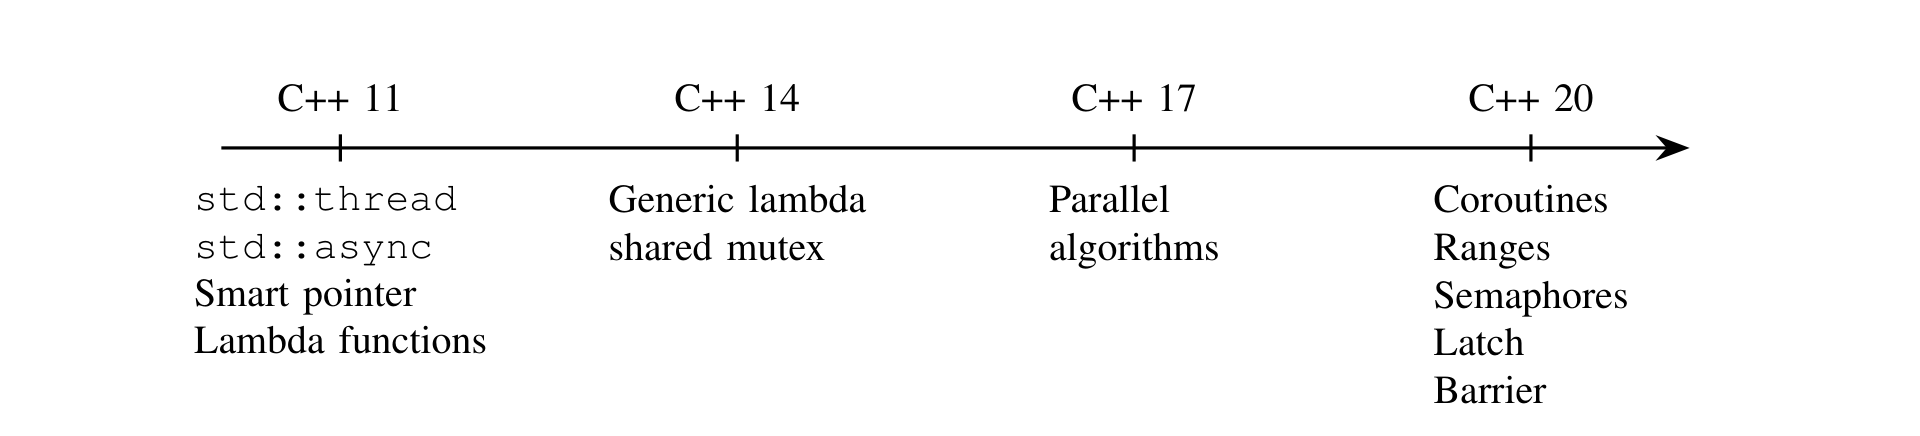
\includegraphics[width=0.95\textwidth]{figures/fig_timeline.png}
  \caption{Dòng thời gian các tính năng song song được bổ sung vào chuẩn C++.
  Nguồn: bài báo \cite{diehl2026}, phỏng theo \cite{diehl2023shared}.}
  \label{fig:timeline}
\end{figure}

\subsubsection{C++11: luồng và lập trình bất đồng bộ}

C++11 đưa vào \code{std::thread}, \code{std::async}, \code{std::future},
\code{std::promise}, lambda và con trỏ thông minh. Trong mô hình bất đồng bộ,
một hàm hoặc lambda được chạy trên một luồng riêng; kết quả được chuyển về qua
đối tượng \code{std::future<T>}. Lời gọi \code{future.get()} sẽ chờ đến khi kết
quả sẵn sàng và trả về giá trị, hoặc ném lại ngoại lệ đã xảy ra trong luồng bất
đồng bộ.

\begin{lstlisting}[language=C++,caption={Mẫu bất đồng bộ với \code{std::async} và \code{std::future}.},label={lst:async}]
std::vector<std::future<void>> tasks;
for (int t = 0; t < nthreads; ++t)
    tasks.push_back(std::async(std::launch::async,
        [&, t] { render_rows(t, nthreads); }));
for (auto& f : tasks) f.get();   // cho tat ca hoan thanh
\end{lstlisting}

Ba đặc điểm cần lưu ý. Thứ nhất, \code{std::async} không bảo đảm mỗi tác vụ có
một luồng riêng; nó có thể dùng thread pool hoặc trì hoãn (\code{launch::deferred}).
Thứ hai, hủy một \code{std::future} từ \code{std::async} có thể chặn cho tới khi
tác vụ kết thúc, nên vòng đời đối tượng quan trọng hơn tưởng tượng. Thứ ba, C++11
không cung cấp API chuẩn để đặt số luồng toàn cục; việc điều khiển số luồng phụ
thuộc hoàn toàn vào cách người lập trình chia tác vụ.

\subsubsection{C++17: thuật toán song song}

C++17 mở rộng thư viện thuật toán bằng execution policy trong header
\code{<execution>}:
\begin{itemize}
  \item \code{std::execution::seq} — thực thi tuần tự;
  \item \code{std::execution::par} — thực thi song song;
  \item \code{std::execution::par\_unseq} — song song, cho phép vector hóa.
\end{itemize}
Ví dụ, \code{std::transform(std::execution::par, ...)}
cho phép thư viện tự chia vòng lặp cho nhiều luồng.

Điểm cốt lõi — và cũng là nguồn lỗi chính trong bài báo — là chuẩn C++ \emph{không}
quy định cách hiện thực execution policy. Với GCC/libstdc++, backend mặc định cho
thuật toán song song là Intel TBB, không phải OpenMP. Do đó, biến môi trường
\code{OMP\_NUM\_THREADS} không điều khiển được số luồng của
\code{std::execution::par}. Muốn giới hạn số luồng, phải dùng API riêng của TBB,
chẳng hạn \code{tbb::global\_control}. Đây là kiến thức hệ sinh thái không suy ra
được từ tài liệu chuẩn C++.

\begin{lstlisting}[language=C++,caption={Thuật toán song song C++17 và giới hạn số luồng bằng TBB.},label={lst:par}]
#include <execution>
#include <algorithm>
#include <tbb/global_control.h>

tbb::global_control limit(tbb::global_control::max_allowed_parallelism, nthreads);
std::for_each(std::execution::par, pixels.begin(), pixels.end(),
              [&](Pixel& p) { p.iter = escape(p.cr, p.ci, max_iter); });
\end{lstlisting}

\subsubsection{C++20: coroutine}

Coroutine C++20 là hàm có thể tạm dừng và tiếp tục tại các điểm xác định, không
cần một ngăn xếp riêng cho mỗi lần dừng (\term{stackless}). Ngôn ngữ chỉ cung cấp
ba từ khóa \code{co\_await}, \code{co\_yield}, \code{co\_return}; phần còn lại do
người lập trình định nghĩa: kiểu \code{task}, \code{promise\_type}, scheduler và
cách quản lý vòng đời.

Trình biên dịch biến đổi thân hàm coroutine thành một máy trạng thái. Mỗi lần gọi
tạo ra một \term{coroutine frame} chứa tham số, biến cục bộ và trạng thái tạm
dừng. Đối tượng \code{promise\_type} điều khiển hành vi:

\begin{itemize}
  \item \code{initial\_suspend()}: coroutine dừng ngay khi được gọi hay chạy luôn.
  \item \code{return\_void()} hoặc \code{return\_value(v)}: tương ứng với
        \code{co\_return;} hoặc \code{co\_return v;}.
  \item \code{yield\_value(v)}: tương ứng với \code{co\_yield v;}.
  \item \code{final\_suspend()}: quyết định điều gì xảy ra khi coroutine kết thúc.
  \item \code{unhandled\_exception()}: xử lý ngoại lệ thoát ra khỏi coroutine.
\end{itemize}

Hàm \code{std::coroutine\_handle<>::done()} chỉ trả về \code{true} khi coroutine
đã dừng tại điểm \code{final\_suspend} và đang ở trạng thái treo. Nếu
\code{final\_suspend()} trả về \code{std::suspend\_never}, coroutine tự hủy frame
ngay khi kết thúc; trạng thái “đã xong” có thể không bao giờ quan sát được qua
\code{done()}. Vòng lặp chờ trong Listing~\ref{lst:corobug} vì thế có thể chạy
mãi.

\begin{lstlisting}[language=C++,caption={Vòng lặp chờ \code{done()} không bao giờ kết thúc khi \code{final\_suspend} là \code{suspend\_never}.},label={lst:corobug}]
while (!tasks[i].done()) {
    std::this_thread::yield();
}
\end{lstlisting}

Một coroutine còn có yêu cầu về quyền sở hữu: frame phải được hủy đúng một lần.
Nếu cả cơ chế \code{final\_suspend} lẫn hàm hủy của đối tượng \code{task} đều
giải phóng cùng một work item, chương trình sẽ gặp lỗi giải phóng bộ nhớ hai lần
— thường biểu hiện thành segmentation fault hoặc thông báo
\code{free(): invalid pointer}. Đây là lớp lỗi ngữ nghĩa không thể phát hiện bằng
trình biên dịch.

\subsubsection{So sánh bốn cơ chế}

Bảng~\ref{tab:cppmodels} tóm tắt khác biệt giữa bốn cách biểu diễn song song
trong C++. Cột “kiểm soát số luồng” đặc biệt quan trọng cho thực nghiệm, vì yêu
cầu cấu hình số luồng bằng dòng lệnh là một ràng buộc phi chức năng của prompt.

\begin{table}[H]
\centering
\small
\caption{So sánh các cơ chế song song bộ nhớ chia sẻ trong C++.}
\label{tab:cppmodels}
\begin{tabularx}{\textwidth}{@{}p{2.9cm} p{3.0cm} X p{2.6cm}@{}}
\toprule
\textbf{Cơ chế} & \textbf{Trừu tượng} & \textbf{Đặc điểm và rủi ro} & \textbf{Kiểm soát số luồng} \\
\midrule
C++11 async & Tác vụ và future & Dễ diễn đạt, nhưng vòng đời future và chính sách khởi chạy phức tạp; không có API chuẩn đặt số luồng & Do người lập trình tự chia tác vụ \\
C++17 parallel algorithms & Vòng lặp song song khai báo & Ngắn gọn; hành vi phụ thuộc backend (TBB với GCC); khó kiểm soát lập lịch và số luồng & Qua API backend, không qua chuẩn \\
C++20 coroutines & Tác vụ hợp tác & Linh hoạt nhất nhưng phải tự viết task, promise và scheduler; lỗi vòng đời khó thấy & Do scheduler tự xây dựng \\
OpenMP & Chỉ thị chia vòng lặp & Quen thuộc, hỗ trợ schedule; dễ sai chia sẻ dữ liệu và dễ bỏ qua số luồng & Trực tiếp qua clause hoặc biến môi trường \\
\bottomrule
\end{tabularx}
\end{table}

\subsection{OpenMP}

OpenMP là mô hình lập trình dựa trên chỉ thị (directive-based) cho bộ nhớ chia sẻ.
Mô hình thực thi là fork--join: một luồng chính tạo ra một nhóm luồng tại vùng
song song, các luồng chia việc theo vòng lặp hoặc vùng tác vụ, rồi hội tụ ở cuối
vùng. Với bài toán Mandelbrot, dạng phổ biến là:

\begin{lstlisting}[language=C++,caption={Song song hóa vòng lặp điểm ảnh bằng OpenMP.},label={lst:omp}]
#pragma omp parallel for schedule(static) num_threads(nthreads)
for (int y = 0; y < height; ++y) {
    for (int x = 0; x < width; ++x)
        image[y*width + x] = escape(...);
}
\end{lstlisting}

Số luồng có thể được đặt theo thứ tự ưu tiên sau (giảm dần):
\begin{enumerate}
  \item clause \code{num\_threads};
  \item lời gọi \code{omp\_set\_num\_threads()};
  \item biến môi trường \code{OMP\_NUM\_THREADS};
  \item giá trị mặc định của runtime.
\end{enumerate}
Việc hiểu đúng thứ tự này rất quan trọng khi kiểm tra
xem chương trình có thực sự tôn trọng tham số dòng lệnh hay không. Ngoài ra,
\code{schedule(static)} chia vòng lặp thành các khối đều nhau, trong khi
\code{schedule(dynamic)} cân bằng tải tốt hơn cho Mandelbrot nhưng tăng chi phí
lập lịch; \code{guided} là dung hòa giữa hai cách.

Một hiện tượng cần lưu ý là \term{chia sẻ giả} (false sharing): hai luồng ghi vào
các biến khác nhau nhưng cùng một dòng cache, khiến cache line bị vô hiệu hóa qua
lại. Với ảnh lớn, hiện tượng này thường không đáng kể vì mỗi luồng ghi vào vùng
nhớ cách xa nhau, nhưng nó có thể xuất hiện nếu chia ảnh theo cột hoặc dùng biến
đếm chung.

\subsection{MPI và mô hình lai MPI+OpenMP}

\subsubsection{SPMD và truyền thông}

MPI theo mô hình \term{Single Program, Multiple Data}: mọi tiến trình chạy cùng
một chương trình, mỗi tiến trình có một định danh \code{rank} và biết tổng số
tiến trình \code{size}. Truyền thông điểm--điểm dùng \code{MPI\_Send} và
\code{MPI\_Recv}; truyền thông tập thể dùng \code{MPI\_Bcast}, \code{MPI\_Reduce},
\code{MPI\_Gather}, \code{MPI\_Scatter}, \ldots{} Các thao tác tập thể có ngữ nghĩa
đồng bộ theo nhóm và thường là nguồn chi phí lớn khi số tiến trình tăng.

Với bài toán ảnh, cách phân vùng tự nhiên là chia theo hàng: tiến trình $r$ tính
các hàng thuộc khoảng
\begin{equation}
  y \in \left[\left\lfloor \frac{rH}{P}\right\rfloor,\;
             \left\lfloor \frac{(r+1)H}{P}\right\rfloor\right),
\end{equation}
với $P$ là số tiến trình. Sau khi tính xong, mỗi tiến trình gửi phần ảnh của mình
về tiến trình gốc (\code{root}) bằng \code{MPI\_Gather}; root ghép các mảnh thành
ảnh đầy đủ và ghi ra tệp.

\subsubsection{MPI\_Gather và các lỗi biên}

\code{MPI\_Gather} yêu cầu mọi tiến trình gửi đúng \code{sendcount} phần tử cùng
kiểu dữ liệu, và root nhận đủ \code{sendcount} từ mỗi tiến trình. Nếu số phần tử
gửi không khớp với vùng đệm nhận, hoặc kiểu dữ liệu không tương thích, chương
trình có thể không báo lỗi ngay mà ghi đè bộ nhớ, dẫn tới \code{free(): invalid
pointer} hoặc segmentation fault. Đây là lớp lỗi rất khó truy nguyên vì vị trí
crash không trùng với vị trí sai.

Một lỗi khác liên quan đến đo đạc: nếu bộ đếm thời gian kết thúc được đặt trước
\code{MPI\_Gather}, thời gian truyền thông bị loại khỏi phép đo. Khi đó chương
trình trông “nhanh” hơn nhưng không phản ánh chi phí thật của mô hình phân tán.
Bài báo ghi nhận đúng lỗi này ở mã LLaMA và phải chỉnh lại mốc đo để so sánh công
bằng \cite{diehl2026}.

\subsubsection{Mô hình lai và chi phí}

Mô hình lai dùng MPI giữa các nút và OpenMP trong mỗi nút: một rank MPI trên mỗi
nút, mỗi rank chạy 20 luồng OpenMP trên 20 lõi. Cách này giảm số thông điệp so
với việc dùng một rank cho mỗi lõi, nhưng đòi hỏi cân bằng tải giữa các nút và
xử lý đúng vùng chia sẻ trong mỗi rank. Chi phí tổng quát:
\begin{equation}
  T(P) = T_{\text{tính}}(P) + T_{\text{truyền thông}}(P) + T_{\text{I/O}},
\end{equation}
trong đó $T_{\text{truyền thông}}$ tăng theo số nút và kích thước dữ liệu gom.
Với ảnh $12000\times80000$ điểm ảnh, bản thân việc gom và ghi ảnh đã là một chi
phí đáng kể, nên việc loại I/O khỏi phép đo — như yêu cầu của prompt — là cần
thiết để so sánh phần tính toán thuần.

\subsubsection{Tăng tốc và hiệu suất}

Với cùng một khối lượng công việc, tăng tốc (speedup) và hiệu suất (efficiency)
được định nghĩa:
\begin{equation}
  S(P) = \frac{T(1)}{T(P)}, \qquad
  E(P) = \frac{S(P)}{P}.
  \label{eq:speedup}
\end{equation}
Định luật Amdahl cho biết nếu tỉ lệ tuần tự là $1-f$ thì
\begin{equation}
  S(P) = \frac{1}{(1-f) + f/P},
  \label{eq:amdahl}
\end{equation}
nên phần tuần tự đặt ra trần tăng tốc. Định luật Gustafson xét bài toán lớn dần
theo số đơn vị xử lý:
\begin{equation}
  S(P) = (1-f) + fP.
  \label{eq:gustafson}
\end{equation}
Trong báo cáo, phép đo mở rộng mạnh (strong scaling) giữ nguyên kích thước ảnh và
tăng số lõi/nút; phép đo mở rộng yếu (weak scaling) không được thực hiện. Vì vậy,
các đường cong tăng tốc cần được đọc cùng với kích thước bài toán và chi phí I/O.

\subsection{LLM và bài toán sinh mã}

LLM là mô hình xác suất dự đoán token tiếp theo trong một chuỗi, được huấn luyện
trên khối lượng lớn văn bản và mã nguồn. Với bài toán sinh mã, mô hình nhận một
prompt và sinh ra chuỗi token; chất lượng phụ thuộc vào dữ liệu huấn luyện, kiến
trúc mô hình, kỹ thuật căn chỉnh và cách diễn đạt prompt. Các thang đo phổ biến
như \term{pass@k} đo xác suất có ít nhất một trong $k$ mẫu sinh vượt qua bộ kiểm
thử, nhưng không phản ánh được các yêu cầu phi chức năng như hiệu năng, khả năng
mở rộng hay tính ổn định.

Ba giới hạn thường gặp rất liên quan đến HPC:

\begin{itemize}
  \item \textbf{Ảo giác API}: mô hình có thể gọi hàm hoặc thuộc tính không tồn tại,
        hoặc trộn API của các phiên bản/thư viện khác nhau.
  \item \textbf{Kiến thức toolchain}: mô hình biết cú pháp nhưng không biết trình
        biên dịch cụ thể đang dùng backend nào, phiên bản thư viện nào, hoặc cờ
        biên dịch nào được bật.
  \item \textbf{Tính không tất định}: cùng một prompt có thể cho các chương trình
        khác nhau; đánh giá một lần sinh không đại diện cho toàn bộ phân phối đầu
        ra.
\end{itemize}

Bài báo giảm thiểu yếu tố thứ ba bằng cách dùng một prompt cố định cho mọi mô
hình và ghi nhận chính xác lần sinh được đánh giá. Đổi lại, kết quả mang tính
nghiên cứu tình huống (case study) hơn là ước lượng thống kê.

\subsection{Công trình liên quan}

Nghiên cứu về LLM cho HPC đã hình thành một số hướng chính. Bảng~\ref{tab:related}
tóm tắt các công trình tiêu biểu và khoảng trống mà bài báo gốc khai thác.

\begin{table}[H]
\centering
\small
\caption{Các công trình liên quan và trọng tâm.}
\label{tab:related}
\begin{tabularx}{\textwidth}{@{}p{3.0cm} X p{3.4cm}@{}}
\toprule
\textbf{Công trình} & \textbf{Nội dung chính} & \textbf{Giới hạn so với bài báo} \\
\midrule
LLM4HPC \cite{chen2023llm4hpc} & Khung đầu tiên cho HPC: phân tích tương đồng mã, phát hiện song song, hỏi đáp OpenMP & Tập trung vào phân tích, chưa đo mở rộng \\
LLM4VV \cite{munley2024llm4vv} & Tinh chỉnh GPT-4 và CodeLLaMA sinh chỉ thị OpenACC & Chỉ một mô hình chỉ thị \\
HPC-GPT \cite{ding2023hpcgpt} & LLaMA-13B cho quản lý mô hình AI, dữ liệu và phát hiện tranh chấp & Không so sánh đa mô hình lập trình \\
HPC-Coder \cite{nichols2024hpccoder,chaturvedi2025hpccoderv2} & Hoàn thành mã cho OpenMP, MPI, CUDA & Bài toán hoàn thành mã, không phải sinh từ đầu \\
OMPGPT \cite{chen2024ompgpt} & Mô hình chuyên sinh mã OpenMP & Chỉ OpenMP \\
MPIRigen \cite{schneider2024mpirigen} & Mô hình miền chuyên sinh mã MPI & Chỉ MPI \\
Tokompiler \cite{kadosh2023tokompiler} & LLM miền hẹp cho Fortran, C, C++ & Tập trung hoàn thành mã \\
chatHPC \cite{yin2025chathpc} & Chatbot hỗ trợ hỏi đáp và sinh script HPC & Không đánh giá mã song song C++ \\
\bottomrule
\end{tabularx}
\end{table}

Khoảng trống có thể thấy rõ: chưa có nghiên cứu đặt nhiều LLM cạnh nhau trên
cùng một bài toán, cùng một bộ prompt, xuyên suốt từ bộ nhớ chia sẻ đến bộ nhớ
phân tán, và đo cả tính đúng lẫn khả năng mở rộng thực tế. Đặc biệt, coroutine
C++20 — cơ chế mới nhất và đang được các khung như Kokkos, HPX quan tâm — chưa
được đánh giá trong bối cảnh sinh mã tự động. Đây chính là điểm mà
\cite{diehl2026} bổ sung.

\phant{PHƯƠNG PHÁP ĐÁNH GIÁ}\label{sec:phuongphap}

\subsection{Thiết kế tổng thể}

Đơn vị phân tích là một cặp (mô hình ngôn ngữ, biến thể lập trình). Với bốn mô
hình và năm biến thể, thiết kế có $4\times5=20$ chương trình. Mỗi chương trình
được sinh từ một prompt cố định, biên dịch, chạy, sửa lỗi tối thiểu và đo đạc
theo cùng một quy trình. Cách bố trí này cho phép so sánh theo hai chiều: giữa
các mô hình trên cùng một biến thể, và giữa các biến thể trong cùng một mô hình.

\begin{table}[H]
\centering
\small
\caption{Ma trận thực nghiệm: bốn mô hình $\times$ năm biến thể.}
\label{tab:matrix}
\begin{tabularx}{\textwidth}{@{}l *{4}{>{\centering\arraybackslash}X}@{}}
\toprule
\textbf{Biến thể} & \textbf{ChatGPT-4} & \textbf{ChatGPT-5} & \textbf{Claude} & \textbf{LLaMA} \\
\midrule
C++11 bất đồng bộ        & C11 & C11 & C11 & C11 \\
C++17 thuật toán song song & C17 & C17 & C17 & C17 \\
C++20 coroutine          & C20 & C20 & C20 & C20 \\
OpenMP                   & OMP & OMP & OMP & OMP \\
MPI+OpenMP               & MPI & MPI & MPI & MPI \\
\bottomrule
\end{tabularx}
\end{table}

Mỗi ô là một lần sinh độc lập. Bài báo không lặp lại nhiều lần cho mỗi ô, không
thay đổi nhiệt độ hay cách diễn đạt prompt. Hệ quả là kết quả mô tả \emph{một}
mẫu đầu ra tiêu biểu, không phải phân phối đầy đủ của mô hình. Đổi lại, thiết kế
giữ được tính nhất quán: mọi so sánh đều dựa trên cùng một điều kiện sinh mã.

\subsection{Yêu cầu chức năng và tiêu chí chấp nhận}

Mỗi chương trình phải thỏa mãn đồng thời các yêu cầu sau:

\begin{enumerate}[label=\textbf{Y\arabic*.},leftmargin=1.6cm]
  \item Biên dịch được bằng GCC 11.5.0 trên nền Linux của cụm thử nghiệm.
  \item Chạy được với tham số dòng lệnh \code{-t <số luồng>}; riêng bản MPI dùng
        \code{-p <số phân vùng>}.
  \item Xuất ảnh Mandelbrot ra tệp theo định dạng PBM/PGM, không cần thư viện
        đồ họa ngoài.
  \item In thời gian chạy \emph{không bao gồm} I/O.
  \item Cho kết quả hình ảnh đúng: tập Mandelbrot hiện rõ, không đen toàn bộ,
        không lệch màu do sai định dạng.
\end{enumerate}

Ba tiêu chí đánh giá được định nghĩa như sau:

\begin{itemize}
  \item \textbf{Biên dịch (build)}: chương trình biên dịch thành công mà không
        cần sửa mã nguồn.
  \item \textbf{Thực thi (runtime)}: chương trình chạy đến khi kết thúc mà không
        treo, không crash, không báo lỗi bộ nhớ.
  \item \textbf{Tính đúng (correctness)}: ảnh đầu ra đúng về mặt trực quan so với
        ảnh tham chiếu.
\end{itemize}

Cần nhấn mạnh rằng “biên dịch được” không kéo theo “chạy đúng”, và “chạy được”
không kéo theo “tôn trọng số luồng”. Ba tiêu chí này độc lập với nhau; khoảng
cách giữa chúng chính là một phần quan trọng của kết quả.

\subsection{Thiết kế prompt}

Ba prompt được dùng nguyên văn cho mọi mô hình. Prompt P1 dùng chung cho ba biến
thể bộ nhớ chia sẻ, chỉ thay phần trong ngoặc nhọn; P2 dùng cho OpenMP; P3 dùng
cho MPI+OpenMP.

\begin{lstlisting}[language={},caption={Prompt P1 -- bộ nhớ chia sẻ với C++11/17/20.},label={lst:p1},numbers=none,basicstyle=\ttfamily\small]
Write a parallel code for the Mandelbrot set using C++ {11 async future,
17 parallel algorithms, 20 coroutines} and write the output to the PBM
format. Make the number of threads configurable with the command line
option -t and print the runtime excluding IO.
\end{lstlisting}

\begin{lstlisting}[language={},caption={Prompt P2 -- OpenMP.},label={lst:p2},numbers=none,basicstyle=\ttfamily\small]
Write a parallel code for the Mandelbrot set using C++ using OpenMP and
write the output to the PBM format. Make the number of threads
configurable with the command line option -t and print the runtime
excluding IO.
\end{lstlisting}

\begin{lstlisting}[language={},caption={Prompt P3 -- MPI+OpenMP.},label={lst:p3},numbers=none,basicstyle=\ttfamily\small]
Write a distributed code using MPI for the Mandelbrot set and using
OpenMP for parallelism in C++ and write the output to the PBM format.
Make the number of partitions configurable with the command line
option -p and print the runtime excluding IO.
\end{lstlisting}

Mỗi mệnh đề trong prompt có một mục đích kiểm thử:

\begin{itemize}
  \item \textbf{“using C++ \{11, 17, 20\}”}: buộc mô hình chọn đúng cơ chế của
        từng phiên bản chuẩn, thay vì dùng OpenMP cho mọi trường hợp.
  \item \textbf{“PBM format”}: tạo đầu ra có thể kiểm tra bằng mắt và bằng tệp,
        đồng thời loại bỏ phụ thuộc vào thư viện đồ họa.
  \item \textbf{“-t” / “-p”}: kiểm tra khả năng phân tích dòng lệnh và — quan
        trọng hơn — khả năng \emph{sử dụng} tham số đó trong phần tính toán.
  \item \textbf{“excluding IO”}: tách chi phí tính toán khỏi chi phí ghi ảnh, cần
        thiết cho phép đo mở rộng.
\end{itemize}

Với MPI, prompt ban đầu chưa đủ. Nếu không nêu rõ “số phân vùng cấu hình được”,
mã sinh ra có xu hướng cho mọi tiến trình tính lại toàn bộ tập Mandelbrot rồi
chỉ ghi phần của mình. Chương trình khi đó trông như song song nhưng không chia
việc, và hiệu năng không tăng theo số nút. Việc bổ sung ràng buộc này là một ví
dụ cụ thể cho thấy chất lượng đặc tả ảnh hưởng trực tiếp đến chất lượng mã.

\subsection{Quy trình kiểm định}

Quy trình gồm năm bước, áp dụng giống nhau cho mọi chương trình:

\begin{enumerate}
  \item \textbf{Biên dịch}: dùng GCC 11.5.0, ghi nhận toàn bộ lỗi và cảnh báo.
  \item \textbf{Sửa lỗi biên dịch}: tác giả sửa với thay đổi tối thiểu, chỉ để
        chương trình biên dịch được; không thiết kế lại thuật toán.
  \item \textbf{Thực thi}: chạy với một luồng và nhiều luồng (hoặc một và nhiều
        tiến trình), kiểm tra treo, crash, lỗi bộ nhớ, kết quả bất thường.
  \item \textbf{Sửa lỗi thực thi}: tiếp tục sửa tối thiểu, ghi lại nguyên nhân
        gốc và cách khắc phục.
  \item \textbf{Kiểm tra tính đúng}: mở ảnh, so sánh trực quan với ảnh tham
        chiếu; với mã MPI, kiểm tra cả trường hợp một tiến trình và nhiều tiến
        trình.
\end{enumerate}

Mỗi lỗi được ghi vào nhật ký với các trường: mô hình, biến thể, loại lỗi (biên
dịch/thực thi/đúng đắn), thông điệp lỗi, nguyên nhân gốc, cách sửa, số dòng thay
đổi và mức độ khó. Cách ghi này cho phép phân loại lỗi ở Phần~\ref{sec:ketqua}
và tách \emph{triệu chứng} khỏi \emph{nguyên nhân}.

Một điểm phương pháp luận cần nêu rõ: sau khi sửa, chương trình được đo hiệu
năng. Vì vậy kết quả mở rộng phản ánh chất lượng của “mã sau sửa”, không phải
chất lượng nguyên bản. Điều này hợp lý nếu mục tiêu là đánh giá năng suất thực
tế — người dùng luôn phải sửa trước khi dùng — nhưng cần tránh diễn giải quá mức
thành “LLM sinh mã chạy đúng ngay”.

\subsection{Độ đo}

\subsubsection{Tỉ lệ thành công}

Với mỗi mô hình, tỉ lệ thành công của từng tiêu chí được tính trên toàn bộ năm
chương trình:
\begin{equation}
  R_{\text{crit}} = \frac{\#\{\text{chương trình đạt tiêu chí crit}\}}{5}\times100\%.
\end{equation}
Cách tính này cho phép so sánh trực tiếp giữa các mô hình, nhưng che khuất sự
khác biệt giữa các biến thể. Vì vậy báo cáo trình bày thêm bảng lỗi chi tiết
theo từng biến thể.

\subsubsection{Kích thước và chi phí mã}

Số dòng mã (LOC) được đo bằng công cụ \code{cloc}, bao gồm cả chú thích, trước
và sau khi sửa. Chi phí phát triển được ước lượng bằng mô hình COCOMO \cite{boehm1984} thông qua
công cụ \code{scc}. Công thức cơ bản của COCOMO:
\begin{equation}
  \text{Effort} = a \cdot (\text{KLOC})^{b},
\end{equation}
với $a,b$ phụ thuộc loại dự án. COCOMO được thiết kế cho phần mềm tuần tự, không
mô hình hóa chi phí đồng bộ, truyền thông hay gỡ lỗi song song. Vì vậy con số
COCOMO chỉ nên đọc như một thước đo tương đối giữa các chương trình cùng loại,
không phải dự báo tuyệt đối.

\subsubsection{Thông lượng và tăng tốc}

Thông lượng được đo bằng số cập nhật điểm ảnh mỗi giây
(\term{pixel updates per second}). Với ảnh $W\times H$ và $I_{\max}$ vòng lặp,
một cách hiểu thận trọng là đại lượng tỉ lệ nghịch với thời gian tính toán của
cùng một khối lượng công việc:
\begin{equation}
  \text{Throughput} \;\propto\; \frac{W\cdot H\cdot I_{\max}}{T_{\text{compute}}}.
\end{equation}
Khi so sánh các đường cong, cần chú ý cả \emph{độ dốc} (khả năng mở rộng) lẫn
\emph{độ cao tuyệt đối} (hiệu năng nền). Một đường phẳng nằm cao có thể là dấu
hiệu chương trình luôn dùng toàn bộ lõi, không phải dấu hiệu mở rộng tốt.

Tăng tốc và hiệu suất được tính theo Công thức~\eqref{eq:speedup}. Với thí
nghiệm phân tán, $P$ là số nút (1, 2, 4, 8, 12), mỗi nút một rank MPI và 20 lõi
OpenMP.

\subsection{Môi trường thực nghiệm}

\begin{table}[H]
\centering
\small
\caption{Cấu hình phần cứng và phần mềm của thực nghiệm.}
\label{tab:env}
\begin{tabularx}{\textwidth}{@{}p{4.2cm} X@{}}
\toprule
\textbf{Thành phần} & \textbf{Cấu hình} \\
\midrule
Cụm & rostam, Đại học Bang Louisiana; phân vùng medusa gồm 16 nút \\
CPU & Intel Xeon Gold 6148 @ 2,40 GHz, 20 lõi/nút \\
Bộ nhớ & 92 GB/nút \\
Trình biên dịch & GCC 11.5.0 \\
MPI & OpenMPI 5.0.7 \\
Backend cho C++17 & Intel TBB 2022.2 \\
Ảnh bộ nhớ chia sẻ & $1920\times1080$ điểm ảnh, 1000 vòng lặp \\
Ảnh phân tán & $12000\times80000$ điểm ảnh, 1000 vòng lặp \\
Cấu hình đo phân tán & 1, 2, 4, 8, 12 nút; 1 rank MPI/nút; 20 lõi/nút \\
Công cụ đo mã & \code{cloc}, \code{scc} \\
\bottomrule
\end{tabularx}
\end{table}

Việc dùng một cấu hình duy nhất giúp so sánh công bằng nhưng giới hạn khả năng
ngoại suy. Kết quả có thể khác trên Clang, trên OpenMP thật (không qua TBB), trên
GPU hoặc trên kiến trúc many-core. Phần~\ref{sec:thaoluan} thảo luận các mối đe
dọa này.

\subsection{Tính tái lập và kiểm soát chất lượng}

Mã sinh ra và mã tham chiếu được công bố trên GitHub và Zenodo \cite{diehl2026}.
Việc công bố cả mã lỗi, bản sửa và ảnh đầu ra cho phép người đọc tái lập từng
bước. Trong quá trình đánh giá, nhóm tác giả giữ nguyên prompt, thứ tự chạy và
cách đo; chỉ thay đổi những dòng cần thiết để chương trình hoạt động. Mọi thay
đổi được ghi lại, nhờ đó có thể phân biệt lỗi của mô hình với can thiệp của con
người.

Một hạn chế cần nêu là mỗi cấu hình chỉ được đo một lần. Bài báo không báo cáo
số lần lặp, độ lệch chuẩn hay khoảng tin cậy. Với các phép đo có biến thiên nhỏ
như thông lượng trung bình trên 20 lõi, sai số có thể chấp nhận được; nhưng với
các điểm gần biên (ví dụ bước nhảy 2$\to$4 nút), cần thận trọng khi diễn giải.
Đây là lý do báo cáo tập trung vào \emph{xu hướng} và \emph{nguyên nhân} hơn là
so sánh chênh lệch nhỏ giữa các đường cong.

\phant{KẾT QUẢ VÀ PHÂN TÍCH}\label{sec:ketqua}

\subsection{Tổng quan tỉ lệ thành công}

Bảng~\ref{tab:success} trình bày tỉ lệ thành công của bốn mô hình trên toàn bộ
năm biến thể. Đây là bảng tổng hợp trung tâm của bài báo: nó cho thấy khoảng cách
lớn giữa “biên dịch được” và “chạy đúng”, đồng thời cho thấy không có mô hình nào
đạt kết quả hoàn hảo ngoài ChatGPT-5.

\begin{table}[H]
\centering
\small
\caption{Tỉ lệ thành công trên toàn bộ chương trình bộ nhớ chia sẻ và phân tán
(Bảng III trong bài báo \cite{diehl2026}).}
\label{tab:success}
\begin{tabular}{@{}lcccc@{}}
\toprule
\textbf{Tiêu chí} & \textbf{ChatGPT-5} & \textbf{ChatGPT-4} & \textbf{Claude} & \textbf{LLaMA} \\
\midrule
Biên dịch   & 100\% & 100\% & 100\% & 40\% \\
Thực thi    & 100\% & 20\%  & 40\%  & 0\% \\
Tính đúng   & 100\% & 100\% & 100\% & 40\% \\
\bottomrule
\end{tabular}
\end{table}

Ba quan sát rút ra từ bảng:

\begin{enumerate}
  \item \textbf{Cú pháp không phải rào cản chính.} Ba trong bốn mô hình biên dịch
        100\% chương trình. Ngay cả LLaMA, mô hình yếu nhất, cũng đạt 40\% — nghĩa
        là phần lớn lỗi không nằm ở cú pháp C++ mà ở ngữ nghĩa song song và kiến
        thức hệ sinh thái.
  \item \textbf{Thực thi là điểm rơi lớn nhất.} ChatGPT-4 biên dịch 100\% nhưng chỉ
        20\% chương trình được tính là chạy không lỗi; Claude đạt 40\%; LLaMA 0\%.
        Đây là bằng chứng định lượng cho luận điểm: mã song song có thể “trông
        đúng” mà vẫn sai ở tầng điều khiển luồng, vòng đời tài nguyên hoặc định
        dạng đầu ra.
  \item \textbf{ChatGPT-5 là mô hình duy nhất đạt 100\% ở cả ba tiêu chí.} Điều
        đáng chú ý là nó không chỉ tránh lỗi mới mà còn sửa đúng các lỗi mà
        ChatGPT-4 mắc phải, cho thấy khả năng nắm bắt ngữ cảnh công cụ tốt hơn.
\end{enumerate}

\noindent\textit{Ghi chú về tính nhất quán của số liệu.} Bảng~\ref{tab:success}
được giữ nguyên theo bài báo, nhưng có vài điểm không khớp hoàn toàn với các bảng
chi tiết. Cụ thể: phần văn bản nói LLaMA thực thi thành công “một chương trình
(20\%)” trong khi Bảng~\ref{tab:success} ghi 0\%; với Claude, bảng tổng hợp ghi
40\% nhưng Bảng I và Bảng II của bài báo đánh dấu thực thi thành công cho ít nhất
ba biến thể (async, OpenMP và MPI), tức 60\%. Ngoài ra, số dòng thêm cho mã
coroutine LLaMA được nêu là 39 ở phần văn bản và 37 ở chú thích Hình~3. Những
điểm này không làm thay đổi kết luận định tính, nhưng cần được lưu ý khi trích
dẫn số liệu.

\subsection{Bộ nhớ chia sẻ: lỗi theo từng mô hình}

\subsubsection{ChatGPT-4: phân tích dòng lệnh và backend}

Với cả bốn biến thể bộ nhớ chia sẻ, ChatGPT-4 in ra hướng dẫn dòng lệnh đầy đủ
như trong Listing~\ref{lst:usage}, nhưng chỉ phân tích tham số \code{-t}. Các
tham số còn lại — kích thước ảnh, số vòng lặp, tâm, tỉ lệ — bị bỏ qua và luôn
dùng giá trị mặc định.

\begin{lstlisting}[language={},caption={Hướng dẫn dòng lệnh do ChatGPT-4 sinh (Listing 1 trong bài báo).},label={lst:usage},numbers=none,basicstyle=\ttfamily\small]
# Usage: [-t threads] [width height [max_iter [x_center y_center [scale]]]]
./exe -t 8 1920 1080 1000 -0.75 0.0 3.0
\end{lstlisting}

Đây là lỗi “đặc tả bề mặt”: chương trình \emph{trông} có giao diện cấu hình, in
ra hướng dẫn đúng, nhưng hành vi thực tế chỉ hỗ trợ một phần. Với phép đo mở rộng,
hệ quả là không thể tăng kích thước ảnh để tạo đủ tải cho 20 lõi nếu không sửa
mã. Nhóm tác giả phải thay đổi kích thước ảnh mặc định để phép đo có ý nghĩa.

Lỗi thứ hai tinh vi hơn. Mã thuật toán song song giả định GCC dùng OpenMP cho
\code{std::execution::par} và đặt biến môi trường \code{OPENMP\_NUM\_THREADS} để
giới hạn số luồng. Thực tế, libstdc++ dùng Intel TBB, nên biến này bị bỏ qua và
chương trình luôn chạy trên toàn bộ lõi. Cách sửa đúng là dùng API TBB, cụ thể
\code{tbb::global\_control} với \code{max\_allowed\_parallelism}. Đây không phải
lỗi cú pháp; nó đòi hỏi kiến thức về backend của thư viện chuẩn trên một trình
biên dịch cụ thể.

\subsubsection{ChatGPT-5: không có lỗi}

ChatGPT-5 không gặp lỗi ở bất kỳ biến thể bộ nhớ chia sẻ nào. Đáng chú ý là nó
phân tích đầy đủ các tham số dòng lệnh — khắc phục lỗi của ChatGPT-4 — và dùng
đúng \code{tbb::global\_control} để giới hạn số luồng. Điều này cho thấy mô hình
không chỉ học cú pháp mà còn học được mẫu tích hợp giữa chuẩn C++ và backend cụ
thể.

\subsubsection{Claude: vòng đời coroutine}

Toàn bộ mã của Claude biên dịch được. Ba biến thể async, thuật toán song song và
OpenMP chạy đúng. Biến thể coroutine treo và không bao giờ kết thúc. Nguyên nhân
là vòng lặp chờ trong Listing~\ref{lst:corobug}: \code{done()} không bao giờ trả
về \code{true} vì coroutine dùng \code{final\_suspend = std::suspend\_never}. Khi
coroutine kết thúc, frame bị hủy ngay; trạng thái “đã hoàn thành” không còn để
quan sát. Đổi sang \code{std::suspend\_always} khắc phục được vấn đề.

Với thuật toán song song, mã sinh ra có một chú thích nhắc người dùng đặt số
luồng, như trong Listing~\ref{lst:comment}. Chú thích này đúng về mặt kỹ thuật,
nhưng bản thân chương trình không thực hiện việc đặt số luồng; nó chỉ ghi nhận
rằng việc đó là cần thiết. Đây là dạng lỗi “biết mà không làm”: mô hình hiểu vấn
đề nhưng không chuyển hiểu biết thành mã.

\begin{lstlisting}[language=C++,caption={Chú thích về số luồng trong mã Claude (Listing 3 trong bài báo).},label={lst:comment}]
/* Set the number of threads for parallel execution
 * Note: C++17 parallel algorithms may not directly use this,
 * but some implementations respect thread pool sizes.
 */
\end{lstlisting}

\subsubsection{LLaMA: chuỗi lỗi chồng chất}

LLaMA là mô hình duy nhất gặp lỗi ở cả bốn biến thể bộ nhớ chia sẻ, và các lỗi có
tính chồng chất: sửa lỗi trước làm lộ lỗi sau.

\begin{itemize}
  \item \textbf{Bất đồng bộ}: chương trình cho ảnh đen với cả một luồng và nhiều
        luồng. Ngoài ra còn lỗi biên dịch \code{std::distance} khi truyền
        \code{Pixel*} thay vì iterator.
  \item \textbf{Thuật toán song song}: hai lỗi biên dịch. Thứ nhất là lỗi
        \code{std::distance} như trên. Thứ hai là việc dùng
        \code{execution\_policy\_tag::concurrency\_hint = numThreads} trong khi
        \code{execution\_policy\_tag} không hề được khai báo — một API không tồn
        tại. Sau khi sửa, chương trình biên dịch nhưng luôn dùng toàn bộ luồng.
  \item \textbf{Coroutine}: ba lớp lỗi. Đầu tiên là promise mismatch: mã dùng
        \code{co\_return} nhưng \code{Task::promise\_type} thiếu
        \code{return\_void()}. Sau khi thêm, chương trình biên dịch nhưng
        segmentation fault do work item bị giải phóng hai lần — một lần bởi
        \code{final\_suspend} và một lần bởi hàm hủy của \code{task}. Sau khi bỏ
        lần giải phóng thứ hai, chương trình chạy nhưng cho ảnh đen vì màu được
        tính theo P5 (8 bit) trong khi ảnh được ghi theo P4 (1 bit). Chỉ sau khi
        đổi định dạng, ảnh mới đúng.
  \item \textbf{OpenMP}: biên dịch được nhưng không tôn trọng số luồng; luôn chạy
        trên toàn bộ lõi hoặc số lõi đặt trước.
\end{itemize}

Chuỗi lỗi này minh họa rõ nhất luận điểm trung tâm của bài báo: lỗi nguy hiểm
nhất trong mã song song không phải lỗi cú pháp, mà là lỗi ngữ nghĩa chỉ biểu hiện
qua hành vi chạy — treo, crash, ảnh sai, hoặc hiệu năng không tăng.

\subsection{Bộ nhớ phân tán: lỗi theo từng mô hình}

Với MPI+OpenMP, bức tranh đơn giản hơn nhưng vẫn lộ ra các vấn đề đặc thù của
truyền thông.

\begin{itemize}
  \item \textbf{ChatGPT-4}: chương trình chạy không lỗi. Tuy nhiên, mã dùng lại
        cùng một hàm tô màu như bản bộ nhớ chia sẻ, không điều chỉnh theo ngữ
        cảnh phân tán. Đây là vấn đề nhất quán chất lượng, không phải lỗi chức
        năng.
  \item \textbf{ChatGPT-5}: biên dịch và chạy thành công, không gặp vấn đề nào.
  \item \textbf{Claude}: chạy đúng như kỳ vọng, không có lỗi.
  \item \textbf{LLaMA}: biên dịch được nhưng chỉ chạy đúng với một tiến trình. Với
        nhiều tiến trình, chương trình crash với \code{free(): invalid pointer};
        sau khi sửa, tiếp tục segmentation fault do lệch vùng đệm trong
        \code{MPI\_Gather}. Ngoài ra, mốc đo thời gian kết thúc được đặt trước
        bước gom dữ liệu, khiến thời gian truyền thông bị loại khỏi phép đo. Phải
        chỉnh lại mốc đo để so sánh công bằng với các mô hình khác.
\end{itemize}

Lỗi \code{MPI\_Gather} của LLaMA là ví dụ điển hình cho lớp lỗi biên: chương
trình không báo lỗi tại dòng gọi MPI, mà crash ở một điểm khác khi bộ nhớ đã bị
ghi đè. Việc tìm ra nguyên nhân đòi hỏi hiểu ngữ nghĩa tham số
\code{sendcount}/\code{recvcount} và kiểu dữ liệu của MPI, chứ không chỉ đọc thông
báo lỗi.

\subsection{Phân loại lỗi và mức độ khó}

Bảng~\ref{tab:errors} tổng hợp các lỗi tiêu biểu, nguyên nhân gốc và cách khắc
phục. Bảng~\ref{tab:taxonomy} phân loại theo tầng và mức độ khó.

\begin{table}[H]
\centering
\small
\caption{Tổng hợp lỗi tiêu biểu và cách khắc phục (rút gọn từ Bảng IV của bài báo).}
\label{tab:errors}
\begin{tabularx}{\textwidth}{@{}p{1.9cm} p{2.1cm} X X@{}}
\toprule
\textbf{Mô hình} & \textbf{Biến thể} & \textbf{Lỗi quan sát} & \textbf{Cách khắc phục} \\
\midrule
ChatGPT-4 & Tất cả & Chỉ \code{-t} được phân tích; các tham số khác bị bỏ qua & Bổ sung phân tích dòng lệnh \\
ChatGPT-4 & Song song & Giả định GCC dùng OpenMP; đặt \code{OPENMP\_NUM\_THREADS} nhưng backend là TBB & Dùng \code{tbb::global\_control} \\
ChatGPT-5 & Tất cả & Không có lỗi & -- \\
Claude & Coroutine & Treo vì \code{done()} không bao giờ \code{true} do \code{final\_suspend = suspend\_never} & Đổi sang \code{suspend\_always} \\
Claude & Song song & Chỉ có chú thích nhắc đặt số luồng, không thực hiện & Đặt số luồng qua TBB \\
LLaMA & Bất đồng bộ & Ảnh đen; lỗi biên dịch \code{std::distance} & Sửa kiểu iterator \\
LLaMA & Song song & \code{std::distance} sai; \code{execution\_policy\_tag} chưa khai báo & Bỏ biến không tồn tại, sửa lời gọi \\
LLaMA & Coroutine & Promise mismatch; segfault do giải phóng hai lần; ảnh đen do P5 ghi vào P4 & Thêm \code{return\_void}, bỏ giải phóng thứ hai, đổi định dạng \\
LLaMA & MPI+OpenMP & \code{free(): invalid pointer}; segfault do lệch buffer \code{MPI\_Gather}; đo thời gian sai & Sửa cấp phát/buffer; chỉnh mốc đo \\
\bottomrule
\end{tabularx}
\end{table}

\begin{table}[H]
\centering
\small
\caption{Phân loại lỗi theo tầng, cách phát hiện và kiến thức cần có.}
\label{tab:taxonomy}
\begin{tabularx}{\textwidth}{@{}p{2.5cm} X p{3.1cm} p{2.2cm}@{}}
\toprule
\textbf{Tầng lỗi} & \textbf{Ví dụ quan sát} & \textbf{Cách phát hiện} & \textbf{Kiến thức cần} \\
\midrule
Cú pháp & \code{std::distance} sai kiểu; biến chưa khai báo & Trình biên dịch & C++ cơ bản \\
API / thư viện & \code{execution\_policy\_tag} không tồn tại; dùng \code{OPENMP\_NUM\_THREADS} cho TBB & Biên dịch hoặc đo số luồng & Hệ sinh thái, phiên bản thư viện \\
Ngữ nghĩa & \code{co\_return} thiếu \code{return\_void}; giải phóng hai lần & Crash, segfault, chạy sai & Vòng đời coroutine, quyền sở hữu \\
Đồng bộ / truyền thông & Lệch buffer \code{MPI\_Gather}; gom dữ liệu sai & Crash khi nhiều tiến trình & Ngữ nghĩa MPI, kích thước buffer \\
Định dạng dữ liệu & Tính màu P5 nhưng ghi P4 & Quan sát ảnh & Đặc tả Netpbm \\
Đo đạc & Kết thúc timer trước \code{MPI\_Gather} & So sánh đường cong bất thường & Phương pháp đo hiệu năng \\
\bottomrule
\end{tabularx}
\end{table}

Có thể xếp mức độ khó như sau. Lỗi cú pháp là dễ nhất: trình biên dịch chỉ đúng
dòng, người sửa chỉ cần biết C++ cơ bản. Lỗi API/thư viện khó hơn: chương trình
vẫn biên dịch, chỉ sai hành vi, nên phải biết backend nào đang chạy. Lỗi ngữ nghĩa
coroutine khó hơn nữa: phải hiểu \code{final\_suspend}, \code{promise\_type} và
quyền sở hữu frame. Lỗi truyền thông MPI khó nhất vì triệu chứng xuất hiện xa
nguyên nhân và phụ thuộc số tiến trình. Lỗi định dạng và lỗi đo đạc nằm ở giữa:
dễ phát hiện nếu có kiểm tra trực quan và so sánh đường cong, nhưng dễ bị bỏ qua
nếu chỉ tin vào “chương trình chạy không crash”.

\subsection{Chất lượng và chi phí mã nguồn}

Hình~\ref{fig:loc} trình bày số dòng mã do \code{cloc} đo được cho bốn biến thể
bộ nhớ chia sẻ. Nhìn chung, ChatGPT-5 và Claude sinh mã dài hơn ChatGPT-4 và
LLaMA. Chỉ với LLaMA, nhóm tác giả phải thêm một lượng đáng kể dòng mới để chương
trình coroutine hoạt động; các mã còn lại chủ yếu sửa vài dòng hiện có.

\begin{figure}[H]
\centering
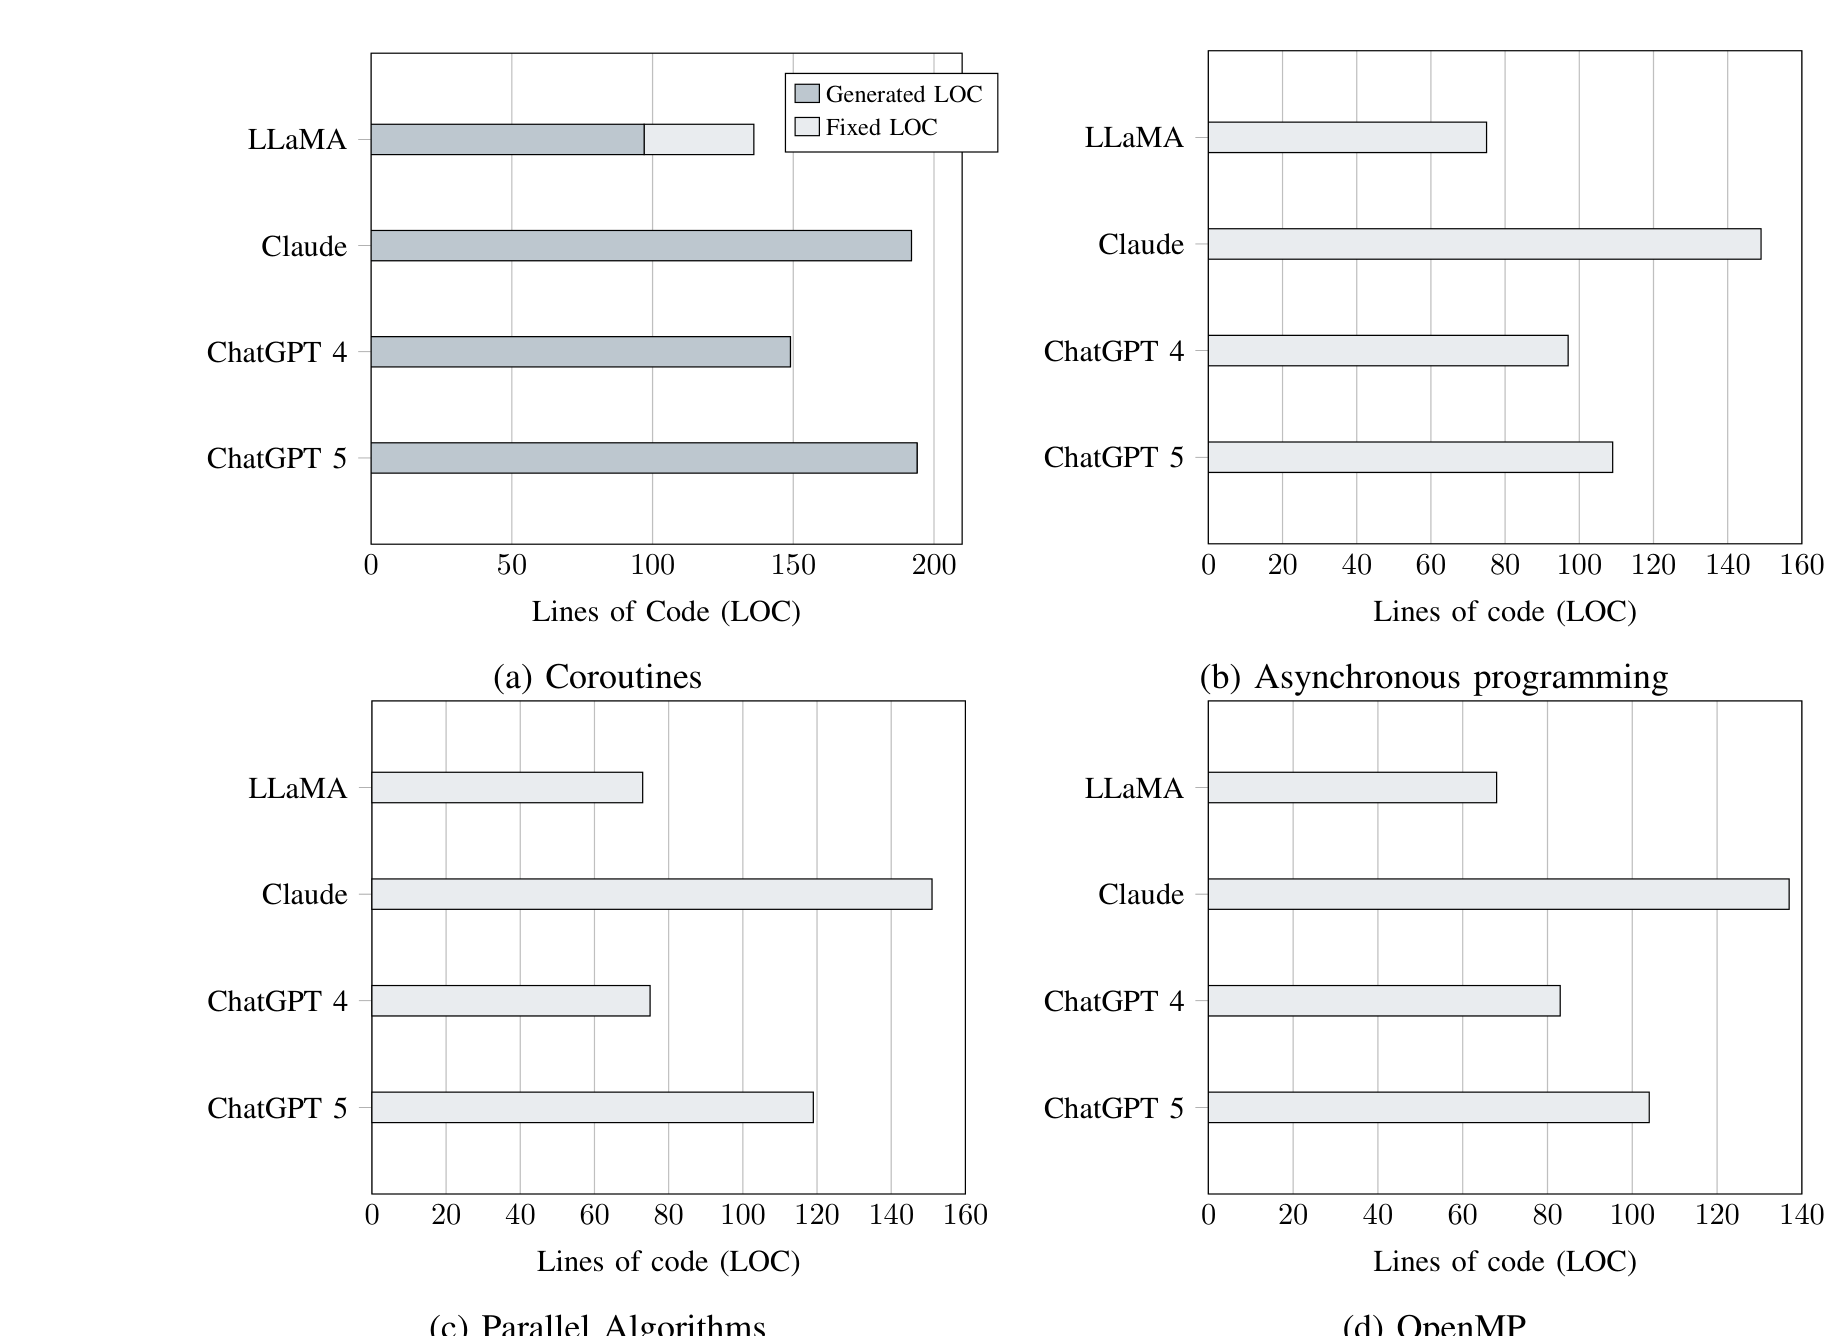
\includegraphics[width=0.92\textwidth]{figures/fig_loc.png}
\caption{Số dòng mã cho bốn biến thể bộ nhớ chia sẻ, trước và sau khi sửa.
Nguồn: bài báo \cite{diehl2026}.}
\label{fig:loc}
\end{figure}

Với bản phân tán, Bảng~\ref{tab:loc} cho thấy ChatGPT-5 sinh nhiều dòng nhất
(143), tiếp theo là Claude (116), ChatGPT-4 (91) và LLaMA (71, sau khi sửa thành
82). Việc phải thêm 11 dòng cho LLaMA cho thấy mã ngắn không đồng nghĩa với mã
tốt: mã càng ngắn càng có thể đã lược bỏ các bước kiểm tra cần thiết.

\begin{table}[H]
\centering
\small
\caption{Số dòng mã cho phiên bản MPI+OpenMP (Bảng V trong bài báo).}
\label{tab:loc}
\begin{tabular}{@{}lcccc@{}}
\toprule
\textbf{Mô hình} & \textbf{ChatGPT-5} & \textbf{ChatGPT-4} & \textbf{Claude} & \textbf{LLaMA} \\
\midrule
LOC & 143 & 91 & 116 & 71 $\to$ 82 \\
\bottomrule
\end{tabular}
\end{table}

Hình~\ref{fig:cocomo} biểu diễn chất lượng và chi phí ước lượng theo COCOMO.
Với bộ nhớ chia sẻ, ChatGPT-5 nằm ở góc “chất lượng tốt, chi phí thấp”; Claude
đứng thứ hai; ChatGPT-4 thứ ba; LLaMA có hai ngoại lệ xấu ở coroutine và thuật
toán song song. Với bộ nhớ phân tán, ChatGPT-5 lại có chi phí ước lượng cao hơn
do số dòng nhiều hơn, còn LLaMA rẻ nhất nhưng cũng là mã duy nhất gặp lỗi thực
thi. Điều này củng cố nhận định: số dòng mã không tỉ lệ nghịch với chất lượng.

\begin{figure}[H]
\centering
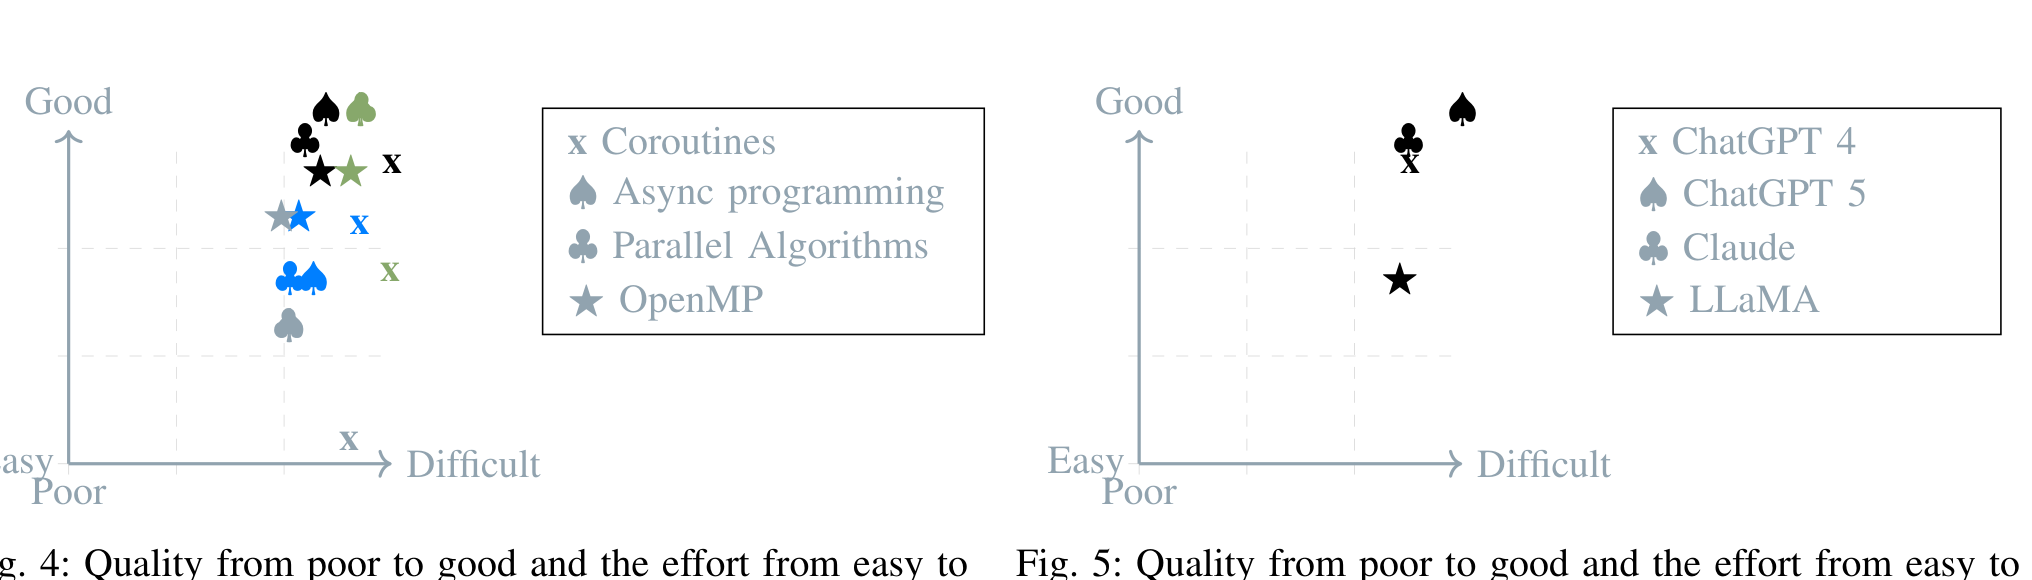
\includegraphics[width=0.98\textwidth]{figures/fig_cocomo.png}
\caption{Chất lượng (trục dọc) và chi phí ước lượng theo COCOMO (trục ngang) cho
mã bộ nhớ chia sẻ (trái) và phân tán (phải). Nguồn: bài báo \cite{diehl2026}.}
\label{fig:cocomo}
\end{figure}

Cần nhấn mạnh giới hạn của COCOMO: mô hình này được xây dựng cho phần mềm tuần
tự, không tính đến chi phí đồng bộ, truyền thông hay gỡ lỗi song song. Vì vậy,
các điểm trên Hình~\ref{fig:cocomo} chỉ nên dùng để so sánh tương đối giữa các
chương trình cùng loại, không nên diễn giải như dự báo nỗ lực tuyệt đối.

\subsection{Khả năng mở rộng trên một nút}

Hình~\ref{fig:scaling} trình bày kết quả mở rộng mạnh trên một nút (tối đa 20
lõi) cho bốn biến thể bộ nhớ chia sẻ. Trục dọc là số cập nhật điểm ảnh mỗi giây
(theo thang logarit), trục ngang là số lõi. Đường màu xanh là mã do con người
viết, dùng làm tham chiếu.

\begin{figure}[H]
\centering
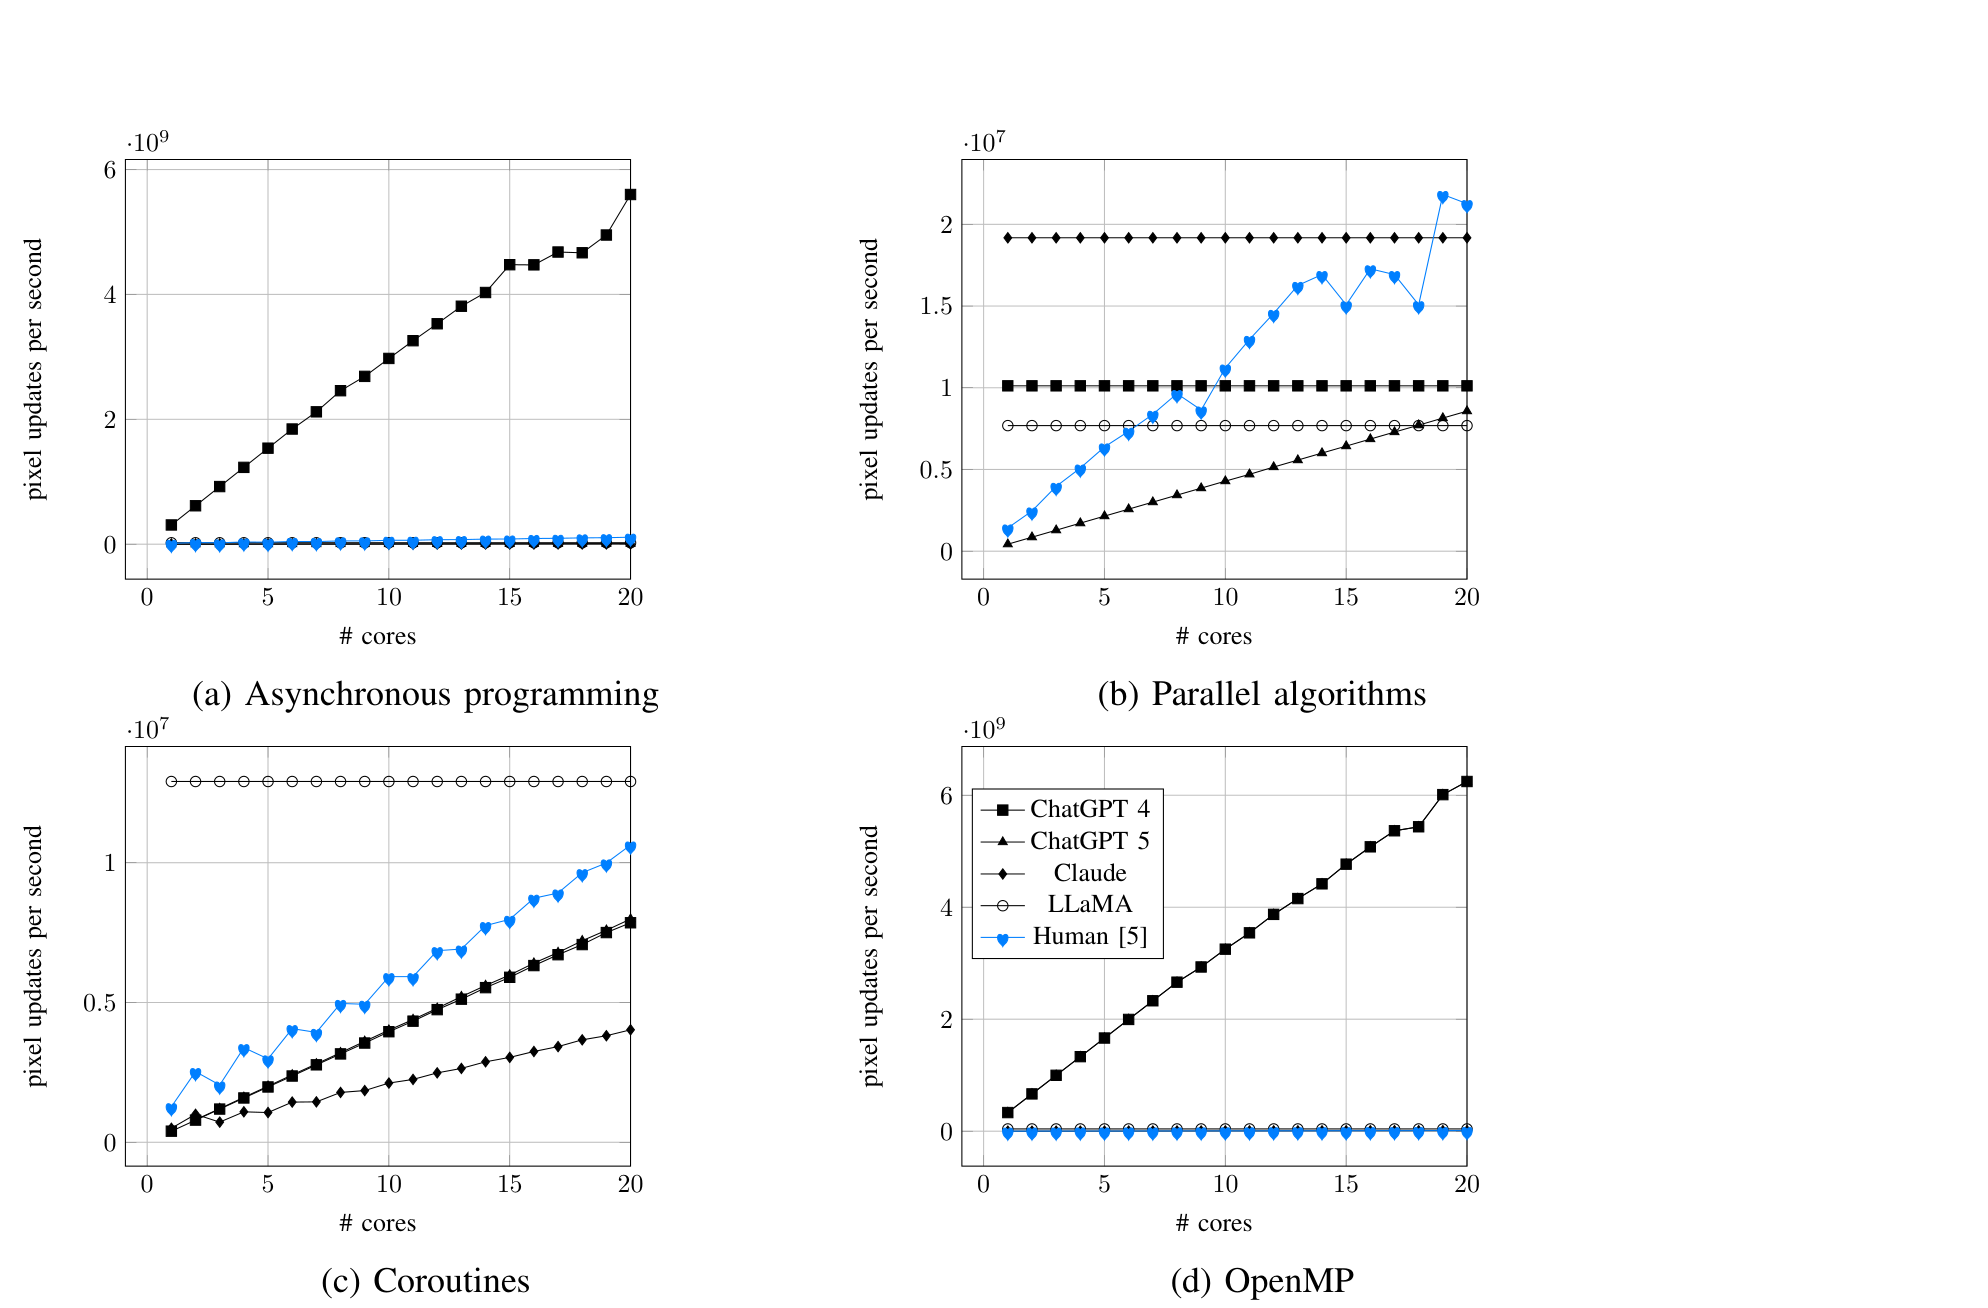
\includegraphics[width=0.95\textwidth]{figures/fig_scaling_shared.png}
\caption{Mở rộng trên một nút: (a) bất đồng bộ, (b) thuật toán song song,
(c) coroutine, (d) OpenMP. Nguồn: bài báo \cite{diehl2026}.}
\label{fig:scaling}
\end{figure}

\subsubsection{Bất đồng bộ}

ChatGPT-4 mở rộng gần tuyến tính đến 15 lõi; sau đó vẫn tăng nhưng chậm dần.
ChatGPT-5 và Claude cũng tăng đến 20 lõi, nhưng thông lượng tuyệt đối thấp hơn
một bậc độ lớn, nên trên thang logarit chúng gần như đường phẳng. LLaMA bỏ qua số
luồng và luôn chạy trên toàn bộ lõi. Điểm đáng chú ý là ChatGPT-4, dù mắc lỗi
phân tích dòng lệnh, lại có phần tính toán bất đồng bộ hiệu quả nhất trong nhóm
LLM — cho thấy lỗi giao diện và lỗi hiệu năng là hai chiều độc lập.

\subsubsection{Thuật toán song song}

ChatGPT-4 luôn dùng đủ 20 lõi bất kể tham số, nên đường biểu diễn là một đường
phẳng nằm ngang. ChatGPT-5 sửa được lỗi này và mở rộng đúng theo số lõi. Claude
và LLaMA cũng bỏ qua tham số số luồng. Đây là minh chứng rõ nhất cho luận điểm
“có tham số không có nghĩa là tôn trọng tham số”: cả bốn chương trình đều nhận
\code{-t}, nhưng chỉ một chương trình thực sự dùng nó để giới hạn backend.

\subsubsection{Coroutine}

ChatGPT-4 và ChatGPT-5 có đường mở rộng gần nhau. Claude cũng mở rộng nhưng chậm
hơn một chút. LLaMA không xét số lõi và nhanh hơn khi dùng toàn bộ lõi, nhưng
điều này không thể hiện khả năng mở rộng có kiểm soát. So với mã con người, cả
ba mô hình đều thấp hơn; đây là biến thể mà khoảng cách với chuyên gia lớn nhất.

\subsubsection{OpenMP}

ChatGPT-4 và ChatGPT-5 mở rộng tốt. Claude cũng mở rộng nhưng thông lượng thấp
hơn một bậc độ lớn, nên đường gần phẳng trên thang logarit. LLaMA chạy trên toàn
bộ lõi và chậm hơn một bậc. Đáng chú ý, mã OpenMP của ChatGPT-5 vượt cả mã con
người trong bài báo — một ngoại lệ hiếm hoi mà LLM thắng ở cả tính đúng lẫn hiệu
năng.

\subsection{Khả năng mở rộng phân tán}

Với thí nghiệm phân tán, ảnh được đặt ở kích thước $12000\times80000$ điểm ảnh,
1000 vòng lặp. Mỗi nút chạy một rank MPI và 20 lõi OpenMP; mỗi rank tính một
phân vùng ảnh. Số nút được tăng theo cấp 1, 2, 4, 8, 12. Hình~\ref{fig:scalingdist}
trình bày kết quả.

\begin{figure}[H]
\centering
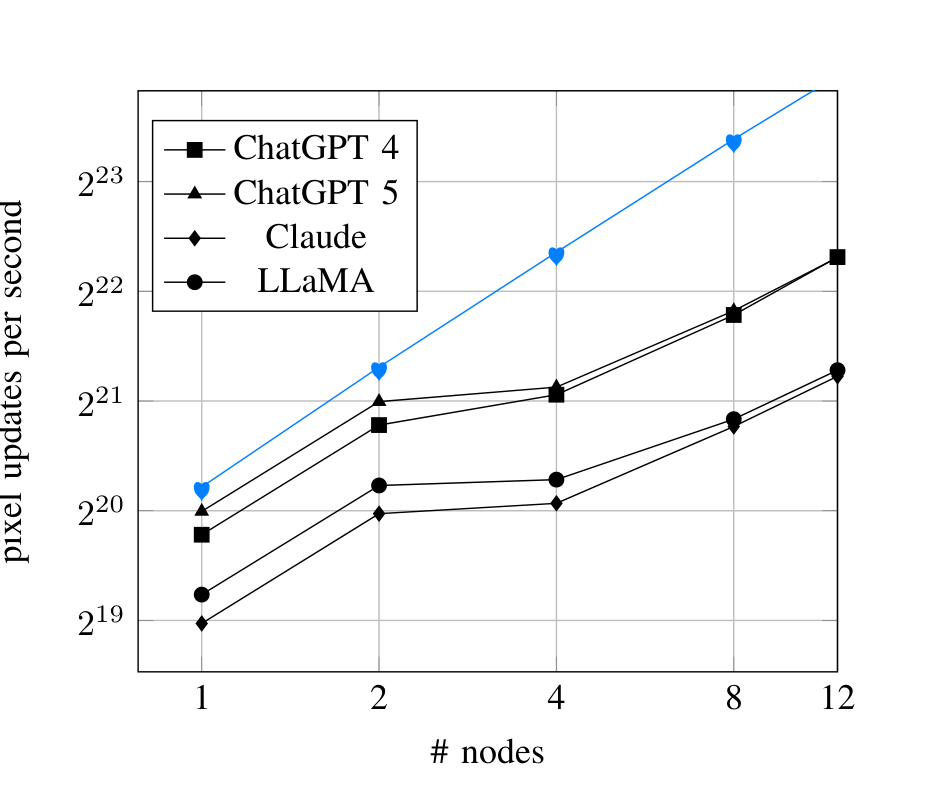
\includegraphics[width=0.62\textwidth]{figures/fig_scaling_dist.png}
\caption{Mở rộng phân tán từ 1 đến 12 nút. Nguồn: bài báo \cite{diehl2026}.}
\label{fig:scalingdist}
\end{figure}

Các quan sát chính:

\begin{itemize}
  \item ChatGPT-4 và ChatGPT-5 đều mở rộng, nhưng tăng tốc từ 2 lên 4 nút thấp
        hơn kỳ vọng; từ 8 lên 12 nút, hai mô hình có hiệu năng tương đương.
  \item Claude mở rộng nhưng chậm hơn hai mô hình OpenAI.
  \item LLaMA, sau khi sửa mốc đo thời gian, mở rộng và có hiệu năng tương đương
        Claude.
  \item Hiện tượng giảm tăng tốc khi đi từ 2 lên 4 nút xuất hiện ở \emph{tất cả}
        các mã, kể cả mã con người. Điều này gợi ý nguyên nhân nằm ở tầng hệ
        thống/truyền thông hơn là ở chất lượng mã do LLM sinh.
  \item Mã con người vẫn dẫn đầu trên toàn dải số nút. Tác giả cho rằng cần phân
        tích sâu hơn các mẫu truyền thông để giải thích khoảng cách này.
\end{itemize}

Điểm đáng khích lệ là sau khi sửa một số lỗi thực thi, \emph{mọi} mã đều mở rộng
được. Điều này cho thấy LLM có thể tạo ra cấu trúc phân tán đúng ở mức khung
(phân vùng, gom dữ liệu, ghi ảnh), ngay cả khi chi tiết biên còn sai. Điểm cần
thận trọng là kết quả chỉ đo một lần cho mỗi cấu hình, nên các chênh lệch nhỏ
giữa các đường cong không nên được diễn giải quá mức.

\subsection{So sánh với mã con người}

Bảng~\ref{tab:human} tóm tắt so sánh giữa mã LLM và mã trong sách
\emph{Parallel C++} \cite{diehl2024book}. Việc chọn mã sách — đã tối ưu nhưng
không tối ưu cực đoan — nhằm tạo một mốc so sánh công bằng, không phải một đối
thủ được huấn luyện riêng cho benchmark.

\begin{table}[H]
\centering
\small
\caption{So sánh tương đối giữa mã LLM và mã con người theo từng biến thể.}
\label{tab:human}
\begin{tabularx}{\textwidth}{@{}p{3.2cm} X p{3.3cm}@{}}
\toprule
\textbf{Biến thể} & \textbf{Kết quả so sánh} & \textbf{Nhận xét} \\
\midrule
Bất đồng bộ & ChatGPT-4 nhanh hơn mã sách nhờ thêm tối ưu & LLM có thể vượt ở mẫu đơn giản \\
Thuật toán song song & Mã sách nhanh hơn ChatGPT-5 & Mã sách mở rộng tốt hơn \\
Coroutine & Mã sách nhanh hơn ChatGPT-4/5 và Claude & Khoảng cách lớn nhất \\
OpenMP & ChatGPT-5 nhanh hơn cả mã sách & Ngoại lệ nổi bật \\
MPI+OpenMP & Mã sách nhanh hơn mọi mã LLM & Cần phân tích truyền thông sâu hơn \\
\bottomrule
\end{tabularx}
\end{table}

Bức tranh tổng thể không đồng nhất. Ở các mẫu đơn giản (async, OpenMP), LLM có
thể ngang hoặc vượt mã sách. Ở các mẫu đòi hỏi điều phối tinh vi (coroutine,
MPI), mã con người vẫn tốt hơn. Điều này phù hợp với giả thuyết rằng LLM mạnh ở
việc tái sử dụng mẫu phổ biến, nhưng yếu ở việc suy luận về vòng đời tài nguyên
và chi phí truyền thông trong một ngữ cảnh cụ thể.

\phant{THẢO LUẬN}\label{sec:thaoluan}

\subsection{Hai lớp kiến thức của mã song song}

Kết quả cho thấy năng lực của LLM trong mã HPC phụ thuộc vào hai lớp kiến thức
khác nhau. Lớp thứ nhất là \emph{cú pháp và thư viện chuẩn}: viết đúng vòng lặp,
đúng chữ ký hàm, đúng cách dùng \code{std::async}, \code{std::execution::par}
hay \code{\#pragma omp parallel for}. Lớp thứ hai là \emph{kiến thức hệ sinh
thái}: trình biên dịch nào, backend nào, phiên bản thư viện nào, tham số nào thực
sự có hiệu lực, và chi phí nào sẽ xuất hiện khi chạy trên phần cứng thật.

Tỉ lệ biên dịch cao (100\% ở ba mô hình) cho thấy lớp thứ nhất đã khá tốt. Khoảng
cách lớn ở tỉ lệ thực thi cho thấy lớp thứ hai còn yếu. Đây là điểm quan trọng
khi đánh giá LLM: một mô hình có thể đạt điểm cao trên các benchmark sinh mã
thuật toán, nơi tiêu chí là “qua bộ kiểm thử”, nhưng vẫn thất bại trong HPC, nơi
tiêu chí là “chạy đúng trên toolchain cụ thể với số tài nguyên cho trước”.

\subsection{Vì sao coroutine là điểm yếu}

Coroutine là biến thể có tỉ lệ lỗi cao nhất và khoảng cách lớn nhất so với mã con
người. Có ba lý do kỹ thuật.

Thứ nhất, coroutine yêu cầu người lập trình tự xây dựng phần hạ tầng: kiểu
\code{task}, \code{promise\_type}, scheduler, cách chờ và cách hủy. Không có một
“task chuẩn” trong C++20. Mỗi chương trình là một thiết kế riêng, nên mỗi lỗi
cũng là một lỗi thiết kế riêng, khó được che chắn bởi các mẫu quen thuộc.

Thứ hai, vòng đời frame là vấn đề ngữ nghĩa, không phải cú pháp. Việc
\code{final\_suspend} trả về \code{suspend\_never} hay \code{suspend\_always}
quyết định ai sở hữu frame, ai hủy nó, và \code{done()} có quan sát được trạng
thái kết thúc hay không. Trình biên dịch không thể cảnh báo vì cả hai lựa chọn
đều hợp lệ về mặt ngôn ngữ; chỉ ngữ cảnh sử dụng mới quyết định đúng sai.

Thứ ba, lỗi coroutine thường biểu hiện muộn: treo, segfault, hoặc ảnh sai. Chúng
không xuất hiện ở dòng khai báo mà ở vòng lặp chờ, ở hàm hủy, hoặc ở bước ghi ảnh.
Việc gỡ lỗi đòi hỏi hiểu luồng thực thi và quyền sở hữu tài nguyên — đúng những
thứ khó suy ra từ một prompt ngắn.

\subsection{“Có tham số” không đồng nghĩa “tôn trọng tham số”}

Một trong những bài học thực tiễn rõ nhất là không nên tin vào giao diện bề mặt.
Nhiều chương trình in ra hướng dẫn dòng lệnh đầy đủ, phân tích \code{-t}, nhưng
không dùng giá trị đó để giới hạn số luồng. Nguyên nhân có thể là:

\begin{itemize}
  \item Backend không phải OpenMP mà là TBB, nên biến môi trường bị bỏ qua.
  \item Số luồng được đặt nhưng thư viện tự quyết định dùng toàn bộ lõi.
  \item Tham số được truyền vào nhưng bị ghi đè bởi giá trị mặc định.
  \item Chương trình dùng song song lồng nhau, và cấp ngoài không bị giới hạn.
\end{itemize}

Cách duy nhất để xác nhận hành vi thật là \emph{đo}. Một phép đo mở rộng đơn giản
— chạy với 1, 2, 4, 8, 16, 20 lõi và vẽ thông lượng — sẽ lộ ra ngay chương trình
nào thực sự tôn trọng tham số. Đây là lý do bài báo không dừng ở kiểm tra biên
dịch mà còn đo hiệu năng.

\subsection{Chất lượng không tỉ lệ với số dòng mã}

Kết quả LOC và COCOMO cho thấy không có quan hệ đơn điệu giữa độ dài mã và chất
lượng. ChatGPT-5 sinh mã dài nhất ở bản phân tán nhưng cũng sạch nhất; LLaMA sinh
mã ngắn nhất nhưng phải thêm dòng và vẫn gặp lỗi thực thi. Mã ngắn có thể đạt được
bằng cách lược bỏ kiểm tra biên, bỏ xử lý lỗi hoặc giả định ngầm về dữ liệu đầu
vào — những thứ chỉ lộ ra khi chạy ở quy mô lớn.

COCOMO cũng cần được đọc thận trọng. Mô hình này ước lượng nỗ lực từ số dòng mã
và các hệ số kinh nghiệm, không mô hình hóa chi phí đồng bộ, truyền thông hay gỡ
lỗi song song. Vì vậy, một chương trình ít dòng hơn không chắc rẻ hơn về tổng chi
phí phát triển; nó chỉ có thể ít dòng hơn. Trong HPC, chi phí gỡ một lỗi
segfault do tranh chấp bộ nhớ có thể lớn hơn nhiều so với chi phí viết thêm vài
chục dòng kiểm tra.

\subsection{Hộp đen và quy mô mô hình}

Bài báo thẳng thắn thừa nhận khó khăn khi giải thích vì sao mô hình này tốt hơn
mô hình khác. LLM là hộp đen: dữ liệu huấn luyện, kiến trúc và chiến lược tối ưu
không được công bố đầy đủ. Có thể giả định dữ liệu huấn luyện chứa nhiều mã nguồn
công khai, nhưng không rõ có bao nhiêu mã song song chất lượng cao, bao nhiêu
thảo luận về TBB, coroutine hay MPI. Quy mô mô hình cũng là yếu tố mờ: các ước
lượng bên ngoài đặt ChatGPT-5 khoảng 600 tỉ tham số, Claude khoảng 175 tỉ, LLaMA
khoảng 400 tỉ, và một số mô hình nhỏ hơn khoảng 31 tỉ. Những con số này không đủ
để giải thích kết quả, vì chất lượng dữ liệu và căn chỉnh quan trọng không kém quy
mô.

Hệ quả phương pháp luận là không nên suy ra “mô hình lớn hơn luôn tốt hơn cho
HPC”. Cần đánh giá trên đúng bài toán, đúng toolchain và đúng tiêu chí. Một mô
hình nhỏ được tinh chỉnh trên mã song song có thể vượt mô hình lớn tổng quát
trong miền hẹp — đây cũng là động lực của các công trình như HPC-Coder, OMPGPT
hay MPIRigen.

\subsection{Hàm ý thực tiễn}

\subsubsection{Khi nào nên dùng LLM cho mã HPC}

Kết quả gợi ý ba mức sử dụng:

\begin{itemize}
  \item \textbf{Phù hợp}: tạo bản nháp cho các mẫu song song quen thuộc (vòng lặp
        OpenMP, async, thuật toán song song), đặc biệt khi bài toán đơn giản và
        có kiểm tra đầu ra rõ ràng.
  \item \textbf{Cần giám sát chặt}: mã coroutine, mã MPI có truyền thông phức
        tạp, mã có quản lý bộ nhớ thủ công. Đây là nơi lỗi ngữ nghĩa tập trung.
  \item \textbf{Chưa nên tin}: các tuyên bố về hiệu năng hoặc khả năng mở rộng
        nếu chưa đo. Không có cách nào thay thế phép đo thực nghiệm.
\end{itemize}

\subsubsection{Quy trình kiểm duyệt đề xuất}

Dựa trên các lỗi quan sát được, có thể áp dụng quy trình năm bước:

\begin{enumerate}
  \item \textbf{Biên dịch với cảnh báo}: bật \code{-Wall -Wextra}, coi cảnh báo
        là lỗi tiềm năng. Lỗi cú pháp là tầng dễ nhất nhưng vẫn cần loại bỏ.
  \item \textbf{Chạy trên dữ liệu nhỏ}: dùng ảnh nhỏ, ít vòng lặp để kiểm tra
        nhanh tính đúng trước khi đo hiệu năng.
  \item \textbf{Kiểm tra đầu ra}: so sánh ảnh với tham chiếu; kiểm tra định dạng
        tệp (P4/P5), kích thước, header.
  \item \textbf{Đo mở rộng}: chạy với nhiều mức lõi/nút, vẽ thông lượng; xác nhận
        tham số số luồng có hiệu lực thật.
  \item \textbf{Soát các điểm ngữ nghĩa}: vòng đời coroutine, quyền sở hữu bộ
        nhớ, kích thước buffer MPI, mốc đo thời gian.
\end{enumerate}

Bảng~\ref{tab:checklist} chuyển các bước này thành danh mục kiểm tra cụ thể.

\begin{table}[H]
\centering
\small
\caption{Danh mục kiểm tra mã song song do LLM sinh.}
\label{tab:checklist}
\begin{tabularx}{\textwidth}{@{}p{2.8cm} X@{}}
\toprule
\textbf{Nhóm} & \textbf{Điểm cần kiểm tra} \\
\midrule
Cú pháp & Biên dịch sạch với \code{-Wall -Wextra}; không dùng API không tồn tại; kiểu iterator đúng \\
Tham số & \code{-t}/\code{-p} được phân tích và \emph{sử dụng}; kiểm tra giá trị biên (0, 1, lớn hơn số lõi) \\
Số luồng & Xác nhận backend (TBB/OpenMP); dùng đúng API giới hạn; đo để chứng minh \\
Coroutine & \code{final\_suspend} phù hợp; \code{promise\_type} có \code{return\_void}/\code{return\_value}; không giải phóng hai lần \\
Bộ nhớ & Cấp phát/giải phóng cân xứng; kiểm tra biên; tránh chia sẻ giả \\
MPI & \code{sendcount}/\code{recvcount} khớp; kiểu dữ liệu khớp; root nhận đủ dữ liệu; xử lý trường hợp $P=1$ \\
Định dạng & Header và dữ liệu cùng định dạng (P4 với 1 bit, P5 với 8 bit); kích thước tệp hợp lệ \\
Đo đạc & Timer bao đúng phần tính toán; loại I/O; ghi rõ số lần lặp và cấu hình \\
Hiệu năng & Đường cong mở rộng có dốc; so sánh với mốc tuần tự; kiểm tra hiệu suất \\
\bottomrule
\end{tabularx}
\end{table}

\subsection{Hạn chế của nghiên cứu}

Có thể phân loại các hạn chế theo bốn mối đe dọa tính hợp lệ.

\subsubsection{Tính hợp lệ về cấu trúc}

Bài toán Mandelbrot là song song hiển nhiên, không có trao đổi dữ liệu giữa các
đơn vị tính toán. Vì vậy, nó không kiểm tra được các lỗi đồng bộ phức tạp, trao
đổi halo, collective nhiều bước hay phụ thuộc dữ liệu — những nơi LLM có thể sai
nhiều hơn. Kết quả về “mã MPI chạy được” chủ yếu nói về khung phân vùng và gom
dữ liệu, không nói về chất lượng của một bộ giải thực thụ.

\subsubsection{Tính hợp lệ nội tại}

Mỗi biến thể chỉ được sinh một lần với một prompt, không lặp lại nhiều lần, không
thay đổi nhiệt độ hay cách diễn đạt. Do đó không có phân tích thống kê về độ biến
thiên. Việc sửa lỗi bởi con người cũng tạo ra yếu tố chủ quan: mức độ “tối thiểu”
của một bản sửa có thể khác nhau giữa các lỗi. Ngoài ra, tiêu chí “ảnh đúng” được
kiểm tra trực quan, không có so sánh điểm ảnh tự động với ảnh tham chiếu.

\subsubsection{Tính hợp lệ bên ngoài}

Thực nghiệm chỉ dùng một trình biên dịch (GCC 11.5.0), một backend (TBB 2022.2),
một nền tảng CPU và một cụm. Kết quả có thể khác trên Clang, trên OpenMP thật,
trên GPU hoặc trên kiến trúc many-core. Bốn mô hình được đánh giá cũng chỉ là một
lát cắt tại thời điểm nghiên cứu; các mô hình mới như Gemini, DeepSeek-Coder hay
Grok chưa được xét.

\subsubsection{Tính hợp lệ của kết luận}

Một số kết luận dựa trên quan sát định tính về hình dạng đường cong, không có
kiểm định thống kê. Các bảng tổng hợp có vài điểm không nhất quán (đã nêu ở
Phần~\ref{sec:ketqua}), nên việc trích dẫn con số cụ thể cần đối chiếu với bảng
chi tiết. Cuối cùng, COCOMO không được thiết kế cho HPC, nên các suy luận về chi
phí chỉ mang tính tương đối.

\phant{KẾT LUẬN VÀ HƯỚNG PHÁT TRIỂN}\label{sec:ketluan}

\subsection{Kết luận}

Nghiên cứu của Diehl, Nader và Gupta đánh giá bốn LLM hàng đầu trên năm biến thể
lập trình song song cho bài toán Mandelbrot. Kết quả cho thấy một bức tranh vừa
lạc quan vừa thận trọng.

Ở mặt tích cực, LLM đã đủ khả năng tạo ra bản nháp mã song song C++ có cấu trúc
đúng. Ba trong bốn mô hình biên dịch 100\% chương trình; sau khi sửa, mọi mã đều
chạy và mở rộng được. ChatGPT-5 đạt 100\% ở cả ba tiêu chí biên dịch, thực thi và
tính đúng — một kết quả đáng chú ý với một bài toán đa mô hình lập trình. Trong
một số trường hợp, mã LLM còn vượt mã con người: bất đồng bộ của ChatGPT-4 và
OpenMP của ChatGPT-5.

Ở mặt hạn chế, khoảng cách giữa “biên dịch được” và “chạy đúng” rất lớn với các
mô hình yếu. ChatGPT-4 biên dịch 100\% nhưng chỉ 20\% chương trình được tính là
chạy không lỗi; Claude đạt 40\%; LLaMA 0\%. Các lỗi tập trung ở ba nhóm: kiểm
soát số luồng (nhầm OpenMP với TBB), vòng đời coroutine (\code{final\_suspend},
\code{promise\_type}, giải phóng hai lần) và định dạng đầu ra (P4/P5). Đây đều là
lỗi ngữ nghĩa hoặc lỗi hệ sinh thái, không phải lỗi cú pháp.

Kết luận trung tâm là: năng lực của LLM trong HPC không nằm ở việc viết đúng cú
pháp, mà ở việc hiểu đúng \emph{ngữ cảnh thực thi} — backend nào, phiên bản nào,
tài nguyên nào, chi phí nào. Khoảng cách lớn nhất so với chuyên gia không phải ở
số dòng mã hay độ phức tạp thuật toán, mà ở hiểu biết về vòng đời tài nguyên và
mô hình truyền thông. Đây là lý do LLM có thể rất hữu ích như trợ lý, nhưng chưa
thể thay thế kỹ sư HPC.

\subsection{Khuyến nghị}

Từ kết quả thực nghiệm, có thể rút ra năm khuyến nghị thực dụng:

\begin{enumerate}
  \item \textbf{Coi mã LLM là bản nháp, không phải sản phẩm.} Luôn biên dịch với
        cảnh báo bật, chạy trên dữ liệu nhỏ và kiểm tra đầu ra trước khi tin
        tưởng.
  \item \textbf{Đo mở rộng thay vì tin vào cờ dòng lệnh.} Kiểm tra backend thực
        tế và xác nhận số luồng có hiệu lực bằng phép đo, không chỉ bằng việc đọc
        mã.
  \item \textbf{Soát kỹ coroutine và MPI.} Với coroutine, kiểm tra
        \code{final\_suspend}, \code{promise\_type} và quyền sở hữu frame. Với
        MPI, kiểm tra kích thước buffer, kiểu dữ liệu, trường hợp một tiến trình
        và mốc đo thời gian.
  \item \textbf{Kiểm tra định dạng đầu ra.} Lỗi P4/P5 có thể tạo ảnh đen mà không
        báo lỗi; cần kiểm tra header, độ sâu bit và kích thước tệp.
  \item \textbf{Viết prompt nêu rõ ràng buộc phi chức năng.} Số luồng/phân vùng
        cấu hình được, đo thời gian loại trừ I/O, định dạng đầu ra, phiên bản
        chuẩn C++, và — với MPI — yêu cầu chia việc thực sự thay vì tính lặp.
\end{enumerate}

Một khuyến nghị ở mức tổ chức: nên xem LLM như một thành viên nhóm cần được
review, không phải một công cụ tự động. Quy trình review cần có danh mục kiểm tra
riêng cho mã song song, vì các tiêu chí thông thường (biên dịch được, qua unit
test) không đủ phát hiện lỗi tôn trọng tài nguyên và lỗi đo đạc.

\subsection{Hướng phát triển}

Bài báo đề xuất nhiều hướng mở rộng, có thể nhóm thành bốn trục.

\subsubsection{Mở rộng bài toán}

Cần đánh giá trên các benchmark truyền thông dày: stencil có trao đổi halo, FFT
song song, bộ giải lặp dùng collective MPI. Đây là nơi lỗi đồng bộ và chi phí
truyền thông thực sự lộ diện. Bên cạnh đó, các ứng dụng khoa học phức tạp như
phần tử hữu hạn hoặc sai phân hữu hạn sẽ kiểm tra khả năng sinh mã cho bài toán
có cấu trúc dữ liệu và phụ thuộc phức tạp.

\subsubsection{Mở rộng mốc so sánh}

Cần so sánh với các phiên bản mã con người được tối ưu cao hơn, không chỉ mã sách
giáo khoa. Đồng thời, nên dùng công cụ profiling và gỡ lỗi để giải thích vì sao
một số mã LLM nhanh hơn hẳn các mã khác — điều mà phép đo thông lượng đơn thuần
không trả lời được.

\subsubsection{Mở rộng mô hình}

Cần bổ sung các mô hình mới như Gemini, DeepSeek-Coder, Grok và các mô hình chuyên
mã. Nên đánh giá nhiều lần sinh cho mỗi cấu hình để có phân tích thống kê, và thử
nghiệm với nhiều cách diễn đạt prompt, nhiệt độ khác nhau. Đây là điều kiện để
chuyển từ nghiên cứu tình huống sang đánh giá có thể khái quát hóa.

Trước khi bổ sung, cần đọc kỹ các nghiên cứu dùng phương pháp thử nghiệm khác —
chẳng hạn đánh giá trên nhiều bài toán thay vì chỉ một bài Mandelbrot — để tránh
so sánh kết quả không cùng điều kiện. Một giả thuyết đáng kiểm chứng là các mô hình
mới khắc phục được phần lớn lỗi cú pháp nhưng vẫn yếu ở khả năng mở rộng;
đây chỉ là giả thuyết, không phải kết luận, vì chưa có phép đo nào trong nghiên cứu
này xác nhận. Cách bổ sung đúng là chạy mô hình mới trên chính ba prompt P1/P2/P3,
biên dịch bằng cùng một toolchain, sửa lỗi tối thiểu theo cùng một quy trình rồi đo
thông lượng trên cùng dải số lõi; khi đó mới có thể thêm một bảng so sánh ngang
hàng và cập nhật kết luận.

\subsubsection{Mở rộng tiêu chí}

Nên so sánh LLM với các công cụ truyền thống như Intel Parallel Advisor, công cụ
phân tích tĩnh và công cụ profiling. Điều này cho thấy LLM bổ sung hay thay thế
những công cụ nào trong quy trình phát triển. Cuối cùng, cần xây dựng bộ tiêu chí
đánh giá mã song song do AI sinh, bao gồm tính đúng, khả năng mở rộng, tính tái
lập và chi phí bảo trì — chứ không chỉ dừng ở tỉ lệ biên dịch.

\subsection{Kết luận cuối}

Bài báo đặt nền móng cho một hướng nghiên cứu còn non trẻ: đánh giá LLM trong bối
cảnh HPC thực thụ. Giá trị lớn nhất của nó không nằm ở việc tuyên bố mô hình nào
“tốt nhất”, mà ở việc chỉ ra \emph{loại lỗi nào} xuất hiện, \emph{vì sao} chúng
xuất hiện, và \emph{cần đo gì} để phát hiện. Đó là nền tảng để xây dựng các quy
trình đánh giá nghiêm túc hơn, các mô hình chuyên biệt hơn, và các công cụ hỗ trợ
lập trình HPC đáng tin cậy hơn trong tương lai.

\clearpage
\section*{PHỤ LỤC A. BẢNG ĐỐI CHIẾU KẾT QUẢ CHI TIẾT}
\addcontentsline{toc}{section}{PHỤ LỤC A. BẢNG ĐỐI CHIẾU KẾT QUẢ CHI TIẾT}

Bảng~\ref{tab:detail} dựng lại kết quả chi tiết của từng biến thể từ Bảng I và
Bảng II trong bài báo. Ký hiệu \checkmark{} là không có lỗi, $\times$ là có lỗi.

\begin{table}[H]
\centering
\small
\caption{Kết quả chi tiết theo biến thể (dựng lại từ Bảng I và II của bài báo).}
\label{tab:detail}
\begin{tabular}{@{}llcccc@{}}
\toprule
\textbf{Biến thể} & \textbf{Tiêu chí} & \textbf{ChatGPT-5} & \textbf{ChatGPT-4} & \textbf{Claude} & \textbf{LLaMA} \\
\midrule
\multirow{3}{*}{Coroutine}
 & Build       & \checkmark & \checkmark & \checkmark & $\times$ \\
 & Runtime     & \checkmark & $\times$   & $\times$   & $\times$ \\
 & Correctness & \checkmark & \checkmark & \checkmark & $\times$ \\
\midrule
\multirow{3}{*}{Bất đồng bộ}
 & Build       & \checkmark & \checkmark & \checkmark & \checkmark \\
 & Runtime     & \checkmark & $\times$   & \checkmark & $\times$ \\
 & Correctness & \checkmark & \checkmark & \checkmark & $\times$ \\
\midrule
\multirow{3}{*}{Thuật toán song song}
 & Build       & \checkmark & \checkmark & \checkmark & $\times$ \\
 & Runtime     & \checkmark & $\times$   & $\times$   & $\times$ \\
 & Correctness & \checkmark & \checkmark & \checkmark & $\times$ \\
\midrule
\multirow{3}{*}{OpenMP}
 & Build       & \checkmark & \checkmark & \checkmark & \checkmark \\
 & Runtime     & \checkmark & $\times$   & \checkmark & $\times$ \\
 & Correctness & \checkmark & \checkmark & \checkmark & $\times$ \\
\midrule
\multirow{3}{*}{MPI+OpenMP}
 & Build       & \checkmark & \checkmark & \checkmark & $\times$ \\
 & Runtime     & \checkmark & \checkmark & \checkmark & $\times$ \\
 & Correctness & \checkmark & \checkmark & \checkmark & $\times$ \\
\bottomrule
\end{tabular}
\end{table}

Bảng~\ref{tab:detail} cho thấy rõ hơn Bảng~\ref{tab:success}: ChatGPT-4 thất bại
ở tầng thực thi cho cả bốn biến thể bộ nhớ chia sẻ, dù không có lỗi biên dịch;
Claude chỉ thất bại ở coroutine và thuật toán song song; LLaMA thất bại ở mọi
tiêu chí ngoài hai lần biên dịch thành công (bất đồng bộ và OpenMP).

\clearpage
\section*{PHỤ LỤC B. KHUNG MPI+OPENMP THAM CHIẾU}
\addcontentsline{toc}{section}{PHỤ LỤC B. KHUNG MPI+OPENMP THAM CHIẾU}

Đoạn mã dưới đây tóm tắt cấu trúc đúng của một chương trình lai MPI+OpenMP cho
bài toán Mandelbrot. Nó không phải mã do LLM sinh, mà là khung tham chiếu để đối
chiếu khi kiểm duyệt. Hai điểm cần chú ý: dùng \code{MPI\_Gatherv} khi số hàng
không chia hết cho số tiến trình, và đặt mốc kết thúc timer \emph{sau} bước gom
dữ liệu nếu muốn đo toàn bộ chi phí.

\begin{lstlisting}[language=C++,caption={Khung MPI+OpenMP với phân vùng theo hàng.},label={lst:mpi},numbers=left]
int rank, size;
MPI_Init(&argc, &argv);
MPI_Comm_rank(MPI_COMM_WORLD, &rank);
MPI_Comm_size(MPI_COMM_WORLD, &size);

int base = height / size;
int local_h = base + (rank < height % size ? 1 : 0);
int y0 = rank * base + std::min(rank, height % size);
std::vector<unsigned char> local(local_h * width);

#pragma omp parallel for schedule(dynamic)
for (int y = 0; y < local_h; ++y)
    for (int x = 0; x < width; ++x)
        local[y*width + x] = escape_pixel(x, y0 + y);

std::vector<int> counts(size), displs(size);
for (int r = 0; r < size; ++r) {
    int h = base + (r < height % size ? 1 : 0);
    counts[r] = h * width;
    displs[r] = (r * base + std::min(r, height % size)) * width;
}

std::vector<unsigned char> image;
if (rank == 0) image.resize(width * height);
MPI_Gatherv(local.data(), (int)local.size(), MPI_UNSIGNED_CHAR,
            image.data(), counts.data(), displs.data(),
            MPI_UNSIGNED_CHAR, 0, MPI_COMM_WORLD);

double t_end = MPI_Wtime();       // do sau khi gather
if (rank == 0) write_pgm("mandel.pgm", image, width, height);
MPI_Finalize();
\end{lstlisting}

\clearpage
\section*{PHỤ LỤC C. CÂU HỎI THẢO LUẬN}
\addcontentsline{toc}{section}{PHỤ LỤC C. CÂU HỎI THẢO LUẬN}

Các câu hỏi dưới đây có thể dùng để thảo luận nhóm hoặc kiểm tra mức hiểu bài.

\begin{enumerate}
  \item Vì sao một chương trình có thể biên dịch 100\% nhưng chỉ 20\% chạy không
        lỗi? Cho ví dụ cụ thể từ bài báo.
  \item GCC dùng backend nào cho \code{std::execution::par}? Vì sao
        \code{OMP\_NUM\_THREADS} không điều khiển được số luồng trong trường hợp
        này?
  \item \code{done()} của coroutine trả về \code{true} khi nào? Điều gì xảy ra
        nếu \code{final\_suspend} là \code{suspend\_never}?
  \item Phân biệt P4 và P5. Vì sao lỗi định dạng có thể tạo ảnh đen mà không báo
        lỗi?
  \item Vì sao \code{MPI\_Gather} có thể gây segfault thay vì báo lỗi ngay? Khi
        nào cần dùng \code{MPI\_Gatherv}?
  \item Đọc một đường cong mở rộng: làm sao phân biệt “mở rộng tốt” với “luôn
        chạy trên toàn bộ lõi”?
  \item COCOMO có phù hợp để đánh giá chi phí phát triển mã HPC không? Vì sao?
  \item Nếu phải chọn một mô hình cho công việc hằng ngày, bạn sẽ dựa trên tiêu
        chí nào ngoài tỉ lệ biên dịch?
\end{enumerate}


\clearpage
\addcontentsline{toc}{section}{TÀI LIỆU THAM KHẢO}
\begin{thebibliography}{99}
\small
\bibitem{diehl2026}
P. Diehl, N. Nader, and D. Gupta, ``LLM-HPC++: Evaluating LLM-Generated Modern
C++ and MPI+OpenMP Codes for Scalable Mandelbrot Set Computation,''
\emph{arXiv:2512.17023v2 [cs.DC]}, Mar. 2026.
DOI: 10.1109/IPDPSW71298.2026.00075.

\bibitem{diehl2024book}
P. Diehl, S. R. Brandt, and H. Kaiser, \emph{Parallel C++: Efficient and Scalable
High-Performance Parallel Programming Using HPX}. Springer Nature, 2024.

\bibitem{diehl2023shared}
P. Diehl, S. R. Brandt, and H. Kaiser, ``Shared Memory Parallelism in Modern C++
and HPX,'' in \emph{Asynchronous Many-Task Systems and Applications}, Springer,
2023, pp. 27--38.

\bibitem{chen2023llm4hpc}
L. Chen, P.-H. Lin, T. Vanderbruggen, C. Liao, M. Emani, and B. De Supinski,
``LLM4HPC: Towards Effective Language Model Application in High-Performance
Computing,'' in \emph{International Workshop on OpenMP}, Springer, 2023,
pp. 18--33.

\bibitem{munley2024llm4vv}
C. Munley, A. Jarmusch, and S. Chandrasekaran, ``LLM4VV: Developing LLM-driven
Testsuite for Compiler Validation,'' \emph{Future Generation Computer Systems},
2024.

\bibitem{ding2023hpcgpt}
X. Ding, L. Chen, M. Emani, C. Liao, P.-H. Lin, T. Vanderbruggen, Z. Xie, A. Cerpa,
and W. Du, ``HPC-GPT: Integrating Large Language Model for High-Performance
Computing,'' in \emph{Proc. SC'23 Workshops}, 2023, pp. 951--960.

\bibitem{nichols2024hpccoder}
D. Nichols et al., ``HPC-Coder: Modeling Parallel Programs using Large Language
Models,'' in \emph{ISC High Performance 2024 Research Paper Proceedings}, 2024,
pp. 1--12.

\bibitem{chaturvedi2025hpccoderv2}
A. Chaturvedi et al., ``HPC-Coder-v2: Studying Code LLMs across Low-Resource
Parallel Languages,'' in \emph{ISC High Performance 2025 Research Paper
Proceedings}, 2025, pp. 1--14.

\bibitem{chen2024ompgpt}
L. Chen, A. Bhattacharjee, N. Ahmed, N. Hasabnis, G. Oren, V. Vo, and A. Jannesari,
``OMPGPT: A Generative Pre-trained Transformer Model for OpenMP,'' in
\emph{European Conference on Parallel Processing}, Springer, 2024, pp. 121--134.

\bibitem{schneider2024mpirigen}
N. Schneider et al., ``MPIRigen: MPI Code Generation through Domain-Specific
Language Models,'' in \emph{Proc. Workshop on AI For Systems}, 2024, pp. 1--6.

\bibitem{kadosh2023tokompiler}
T. Kadosh et al., ``Scope is All You Need: Transforming LLMs for HPC Code,''
\emph{arXiv:2308.09440}, 2023.

\bibitem{yin2025chathpc}
J. Yin et al., ``chatHPC: Empowering HPC Users with Large Language Models,''
\emph{The Journal of Supercomputing}, vol. 81, no. 1, p. 194, 2025.

\bibitem{chen2024landscape}
L. Chen et al., ``The Landscape and Challenges of HPC Research and LLMs,''
\emph{CoRR}, 2024.

\bibitem{lei2023dataset}
B. Lei et al., ``Creating a Dataset for High-Performance Computing Code
Translation using LLMs: A Bridge Between OpenMP Fortran and C++,'' in
\emph{IEEE HPEC}, 2023, pp. 1--7.

\bibitem{godoy2023codex}
W. Godoy, P. Valero-Lara, K. Teranishi, P. Balaprakash, and J. Vetter,
``Evaluation of OpenAI Codex for HPC Parallel Programming Models Kernel
Generation,'' in \emph{Proc. ICPP Workshops}, 2023, pp. 136--144.

\bibitem{valero2023llama}
P. Valero-Lara, A. Huante, M. A. Lail, W. F. Godoy, K. Teranishi,
P. Balaprakash, and J. S. Vetter, ``Comparing Llama-2 and GPT-3 LLMs for HPC
Kernels Generation,'' \emph{arXiv:2309.07103}, 2023.

\bibitem{godoy2024evaluation}
W. F. Godoy et al., ``Large Language Model Evaluation for High-Performance
Computing Software Development,'' \emph{Concurrency and Computation: Practice
and Experience}, vol. 36, no. 26, p. e8269, 2024.

\bibitem{chen2021evaluating}
M. Chen et al., ``Evaluating Large Language Models Trained on Code,''
\emph{arXiv:2107.03374}, 2021.

\bibitem{achiam2023gpt4}
J. Achiam et al., ``GPT-4 Technical Report,'' \emph{arXiv:2303.08774}, 2023.

\bibitem{touvron2023llama}
H. Touvron et al., ``LLaMA: Open and Efficient Foundation Language Models,''
\emph{arXiv:2302.13971}, 2023.

\bibitem{boehm1984}
B. W. Boehm, ``Software Engineering Economics,'' \emph{IEEE Transactions on
Software Engineering}, vol. SE-10, no. 1, pp. 4--21, 1984.

\bibitem{miller2018cocomo}
J. Miller, S. Wienke, M. Schlottke-Lakemper, M. Meinke, and M. S. M\"uller,
``Applicability of the Software Cost Model COCOMO II to HPC Projects,''
\emph{International Journal of Computational Science and Engineering},
vol. 17, no. 3, pp. 283--296, 2018.

\bibitem{brooks1980}
R. Brooks and J. P. Matelski, ``The Dynamics of 2-Generator Subgroups of
PSL(2, $\mathbb{C}$),'' in \emph{Riemann Surfaces and Related Topics: Proc. 1978
Stony Brook Conference}, vol. 97, 1980, pp. 65--71.

\bibitem{mandelbrot2004}
B. B. Mandelbrot, ``Fractal Aspects of the Iteration of $z\to\lambda z(1-z)$ for
Complex $\lambda$ and $z$,'' in \emph{Fractals and Chaos: The Mandelbrot Set and
Beyond}, Springer, 2004, pp. 37--51.

\bibitem{drakopoulos2003}
V. Drakopoulos, N. Mimikou, and T. Theoharis, ``An Overview of Parallel
Visualisation Methods for Mandelbrot and Julia Sets,'' \emph{Computers \&
Graphics}, vol. 27, no. 4, pp. 635--646, 2003.

\bibitem{robey2021}
R. Robey and Y. Zamora, \emph{Parallel and High Performance Computing}. Simon and
Schuster, 2021.

\bibitem{gropp1999}
W. Gropp, E. Lusk, and A. Skjellum, \emph{Using MPI: Portable Parallel Programming
with the Message-Passing Interface}. MIT Press, 1999.

\bibitem{diaz2012}
J. Diaz, C. Munoz-Caro, and A. Nino, ``A Survey of Parallel Programming Models and
Tools in the Multi and Many-Core Era,'' \emph{IEEE Transactions on Parallel and
Distributed Systems}, vol. 23, no. 8, pp. 1369--1386, 2012.

\bibitem{lin2022isocpp}
W.-C. Lin, T. Deakin, and S. McIntosh-Smith, ``Evaluating ISO C++ Parallel
Algorithms on Heterogeneous HPC Systems,'' in \emph{IEEE/ACM PMBS}, 2022,
pp. 36--47.

\bibitem{belson2020coroutines}
B. Belson, W. Xiang, J. Holdsworth, and B. Philippa, ``C++20 Coroutines on
Microcontrollers---What We Learned,'' \emph{IEEE Embedded Systems Letters},
vol. 13, no. 1, pp. 9--12, 2020.

\bibitem{kang2015}
S. J. Kang, S. Y. Lee, and K. M. Lee, ``Performance Comparison of OpenMP, MPI, and
MapReduce in Practical Problems,'' \emph{Advances in Multimedia}, vol. 2015,
p. 575687, 2015.

\end{thebibliography}

\end{document}
